\section{Supplementary Figures}

\begin{figure}[h!]
    \centering
    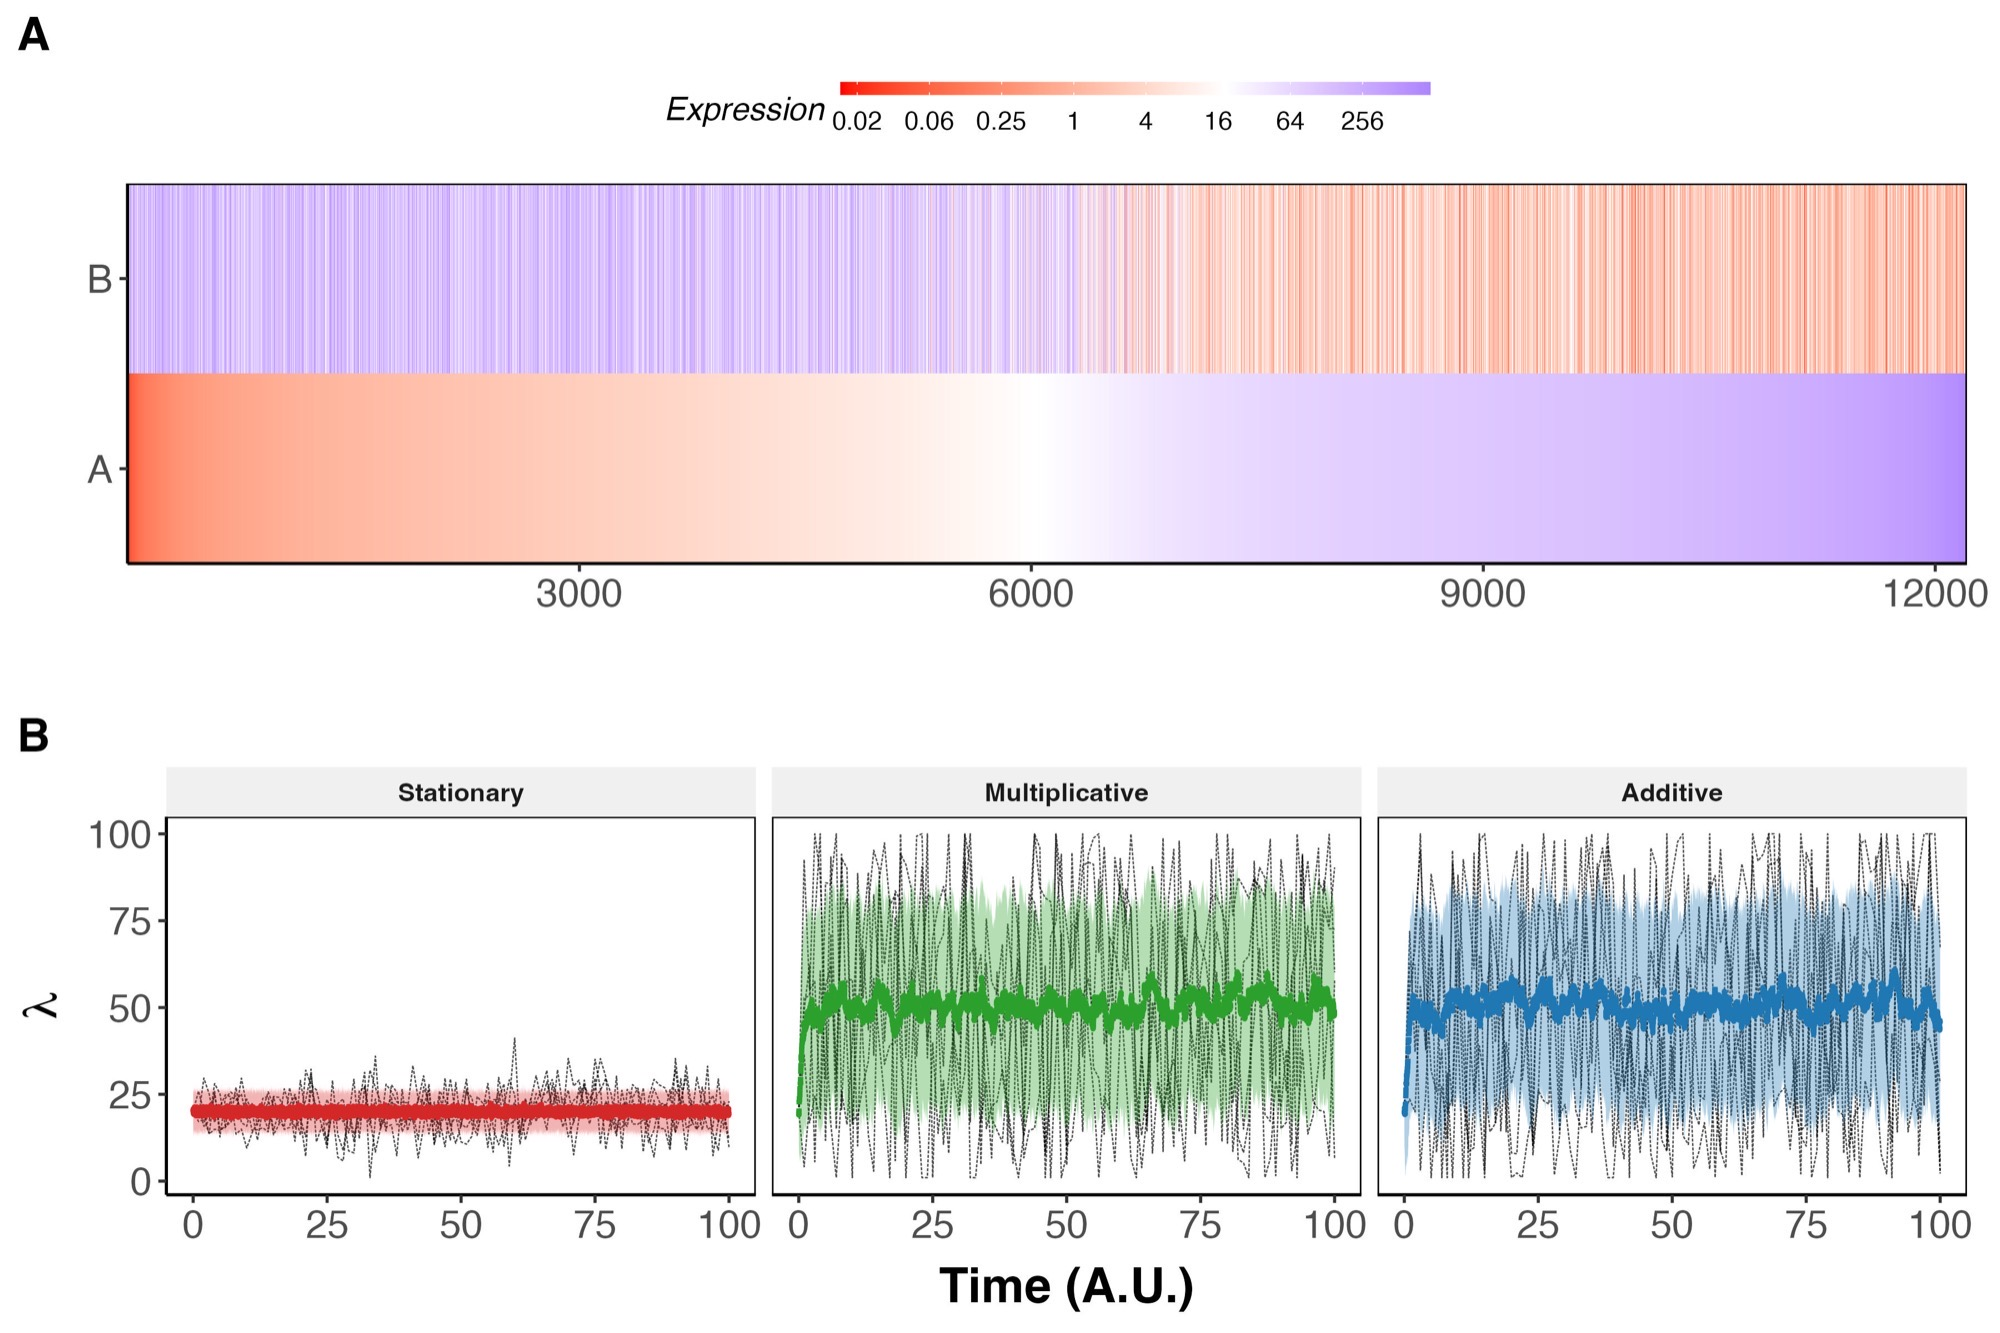
\includegraphics[width=0.8\linewidth]{Fig1S1.jpg}
    \caption{
    \textbf{(A)} Heatmap of RACIPE steady-state expression for nodes A and B in TS network, across all sampled parameter combinations. The steady states are sorted in increasing order of expression of node A. The color scale is in $log_2$ scale and centered at the mean of the two nodes' thresholds. \textbf{(B)} Same design as Figure~\ref{fig:1}D, but for a fold-change of an activatory edge ($\lambda \in [1,100]$, $\lambda_0 = 20$).}
    \label{fig:1S1}
\end{figure}

\begin{figure}
    \centering
    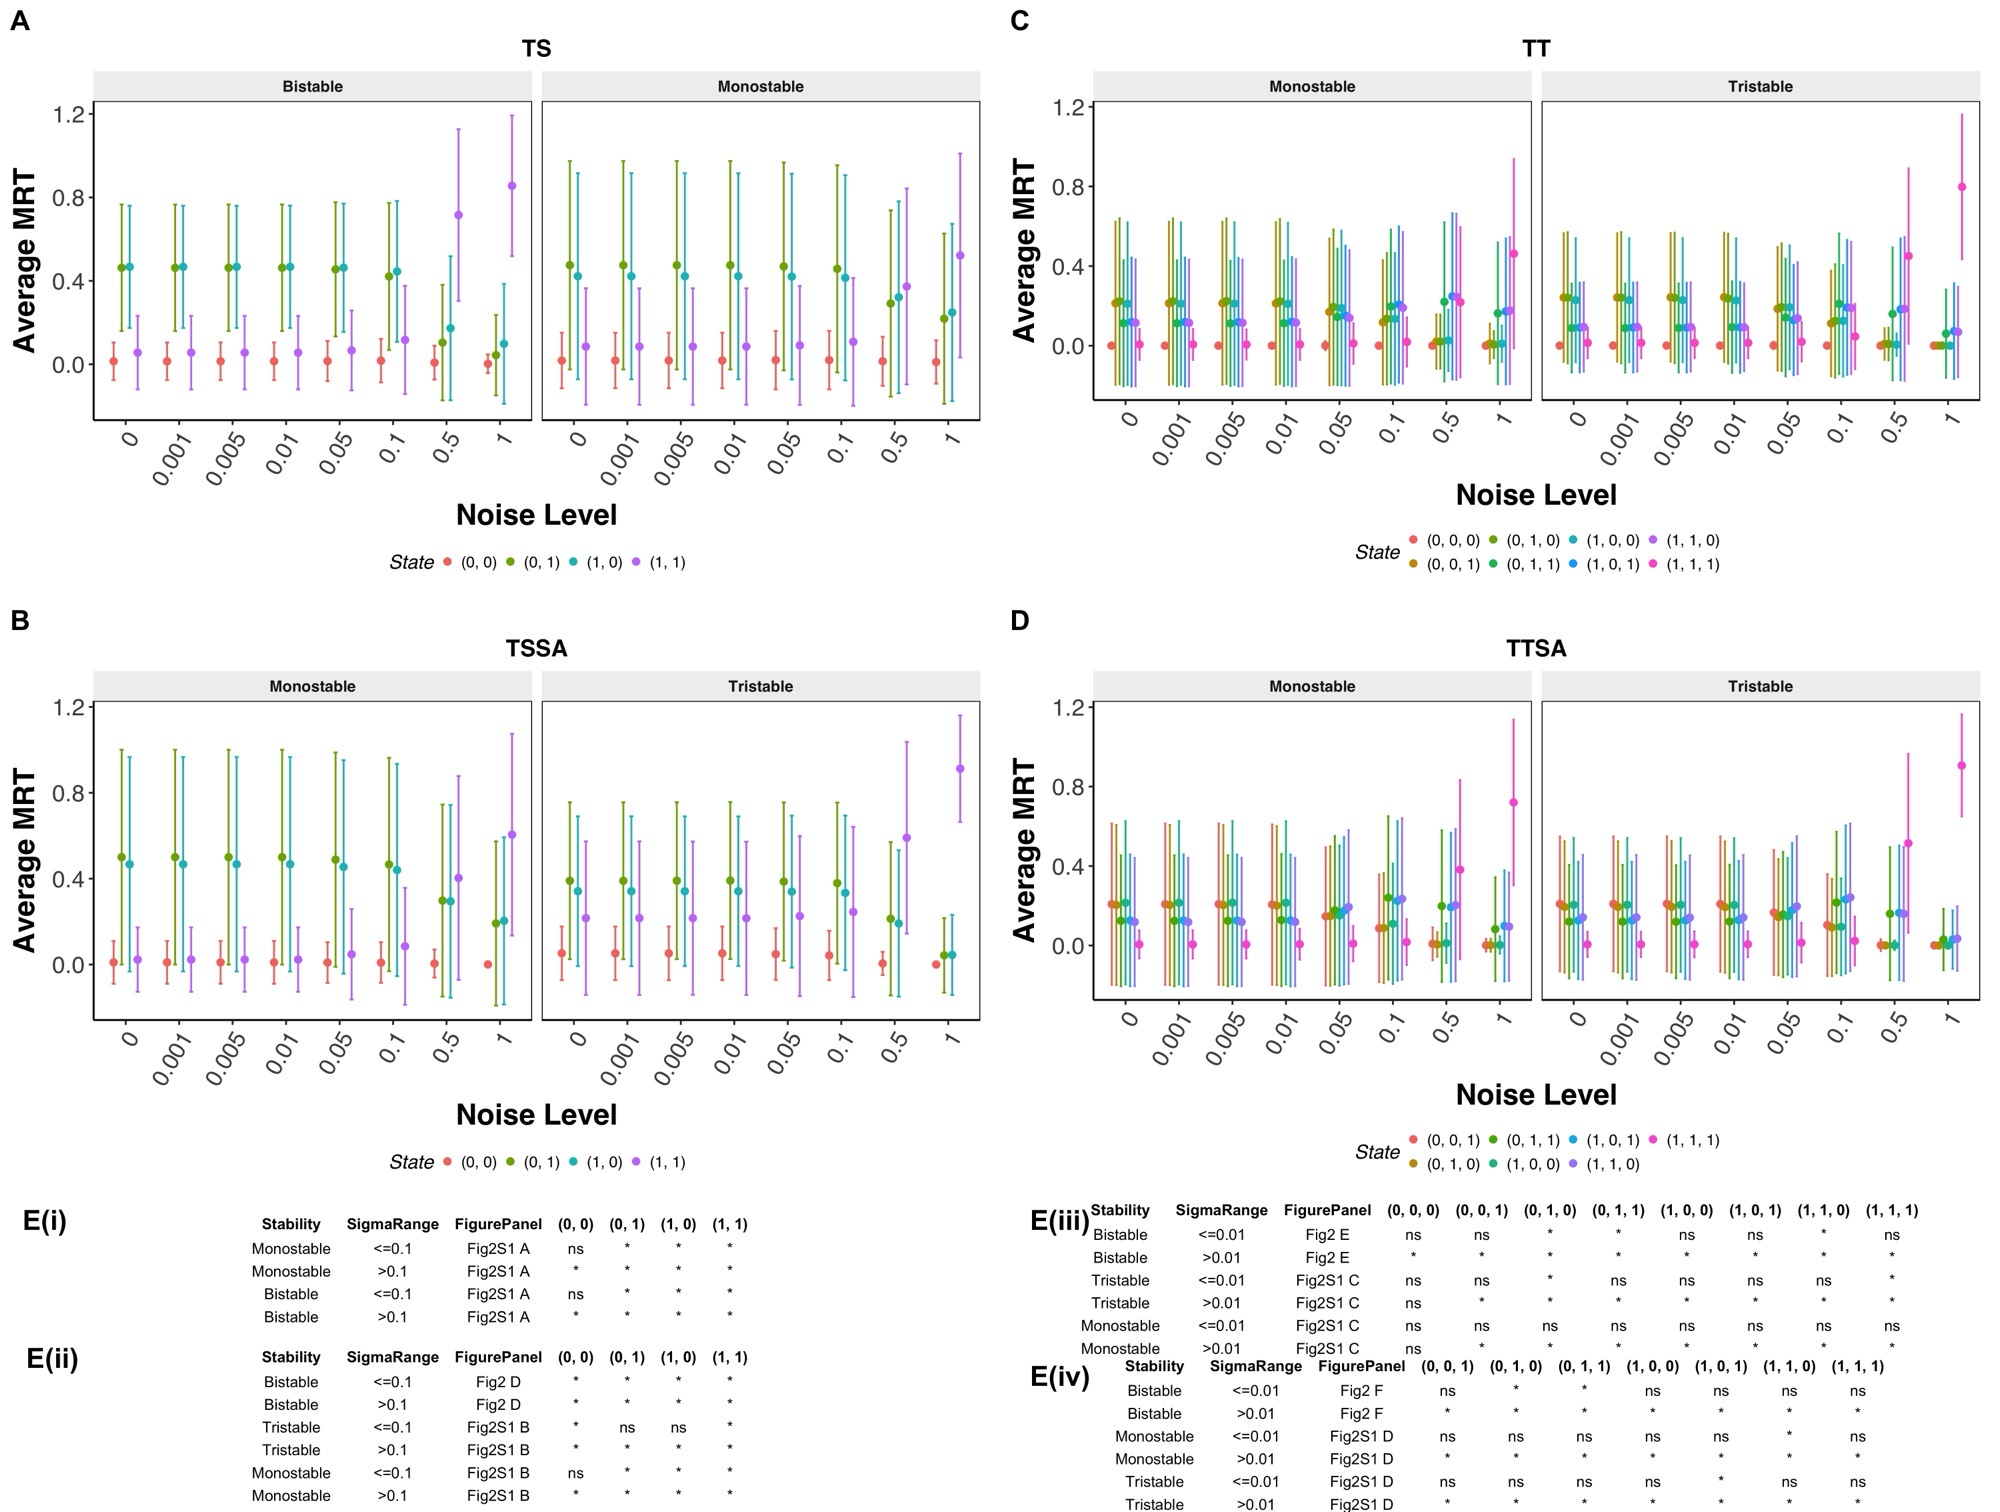
\includegraphics[width=0.8\linewidth]{Fig2S1.jpg}
    \caption{MRT vs.\ noise level, colored by discrete state, mean $\pm$ SD across parameter sets, for \textbf{(A)} TS (all parameter sets), \textbf{(B)} TSSA (monostable + tristable), \textbf{(C)} TT (monostable + tristable), and \textbf{(D)} TTSA (monostable + tristable).}
    \label{fig:2S1}
\end{figure}

\begin{figure}
    \centering
    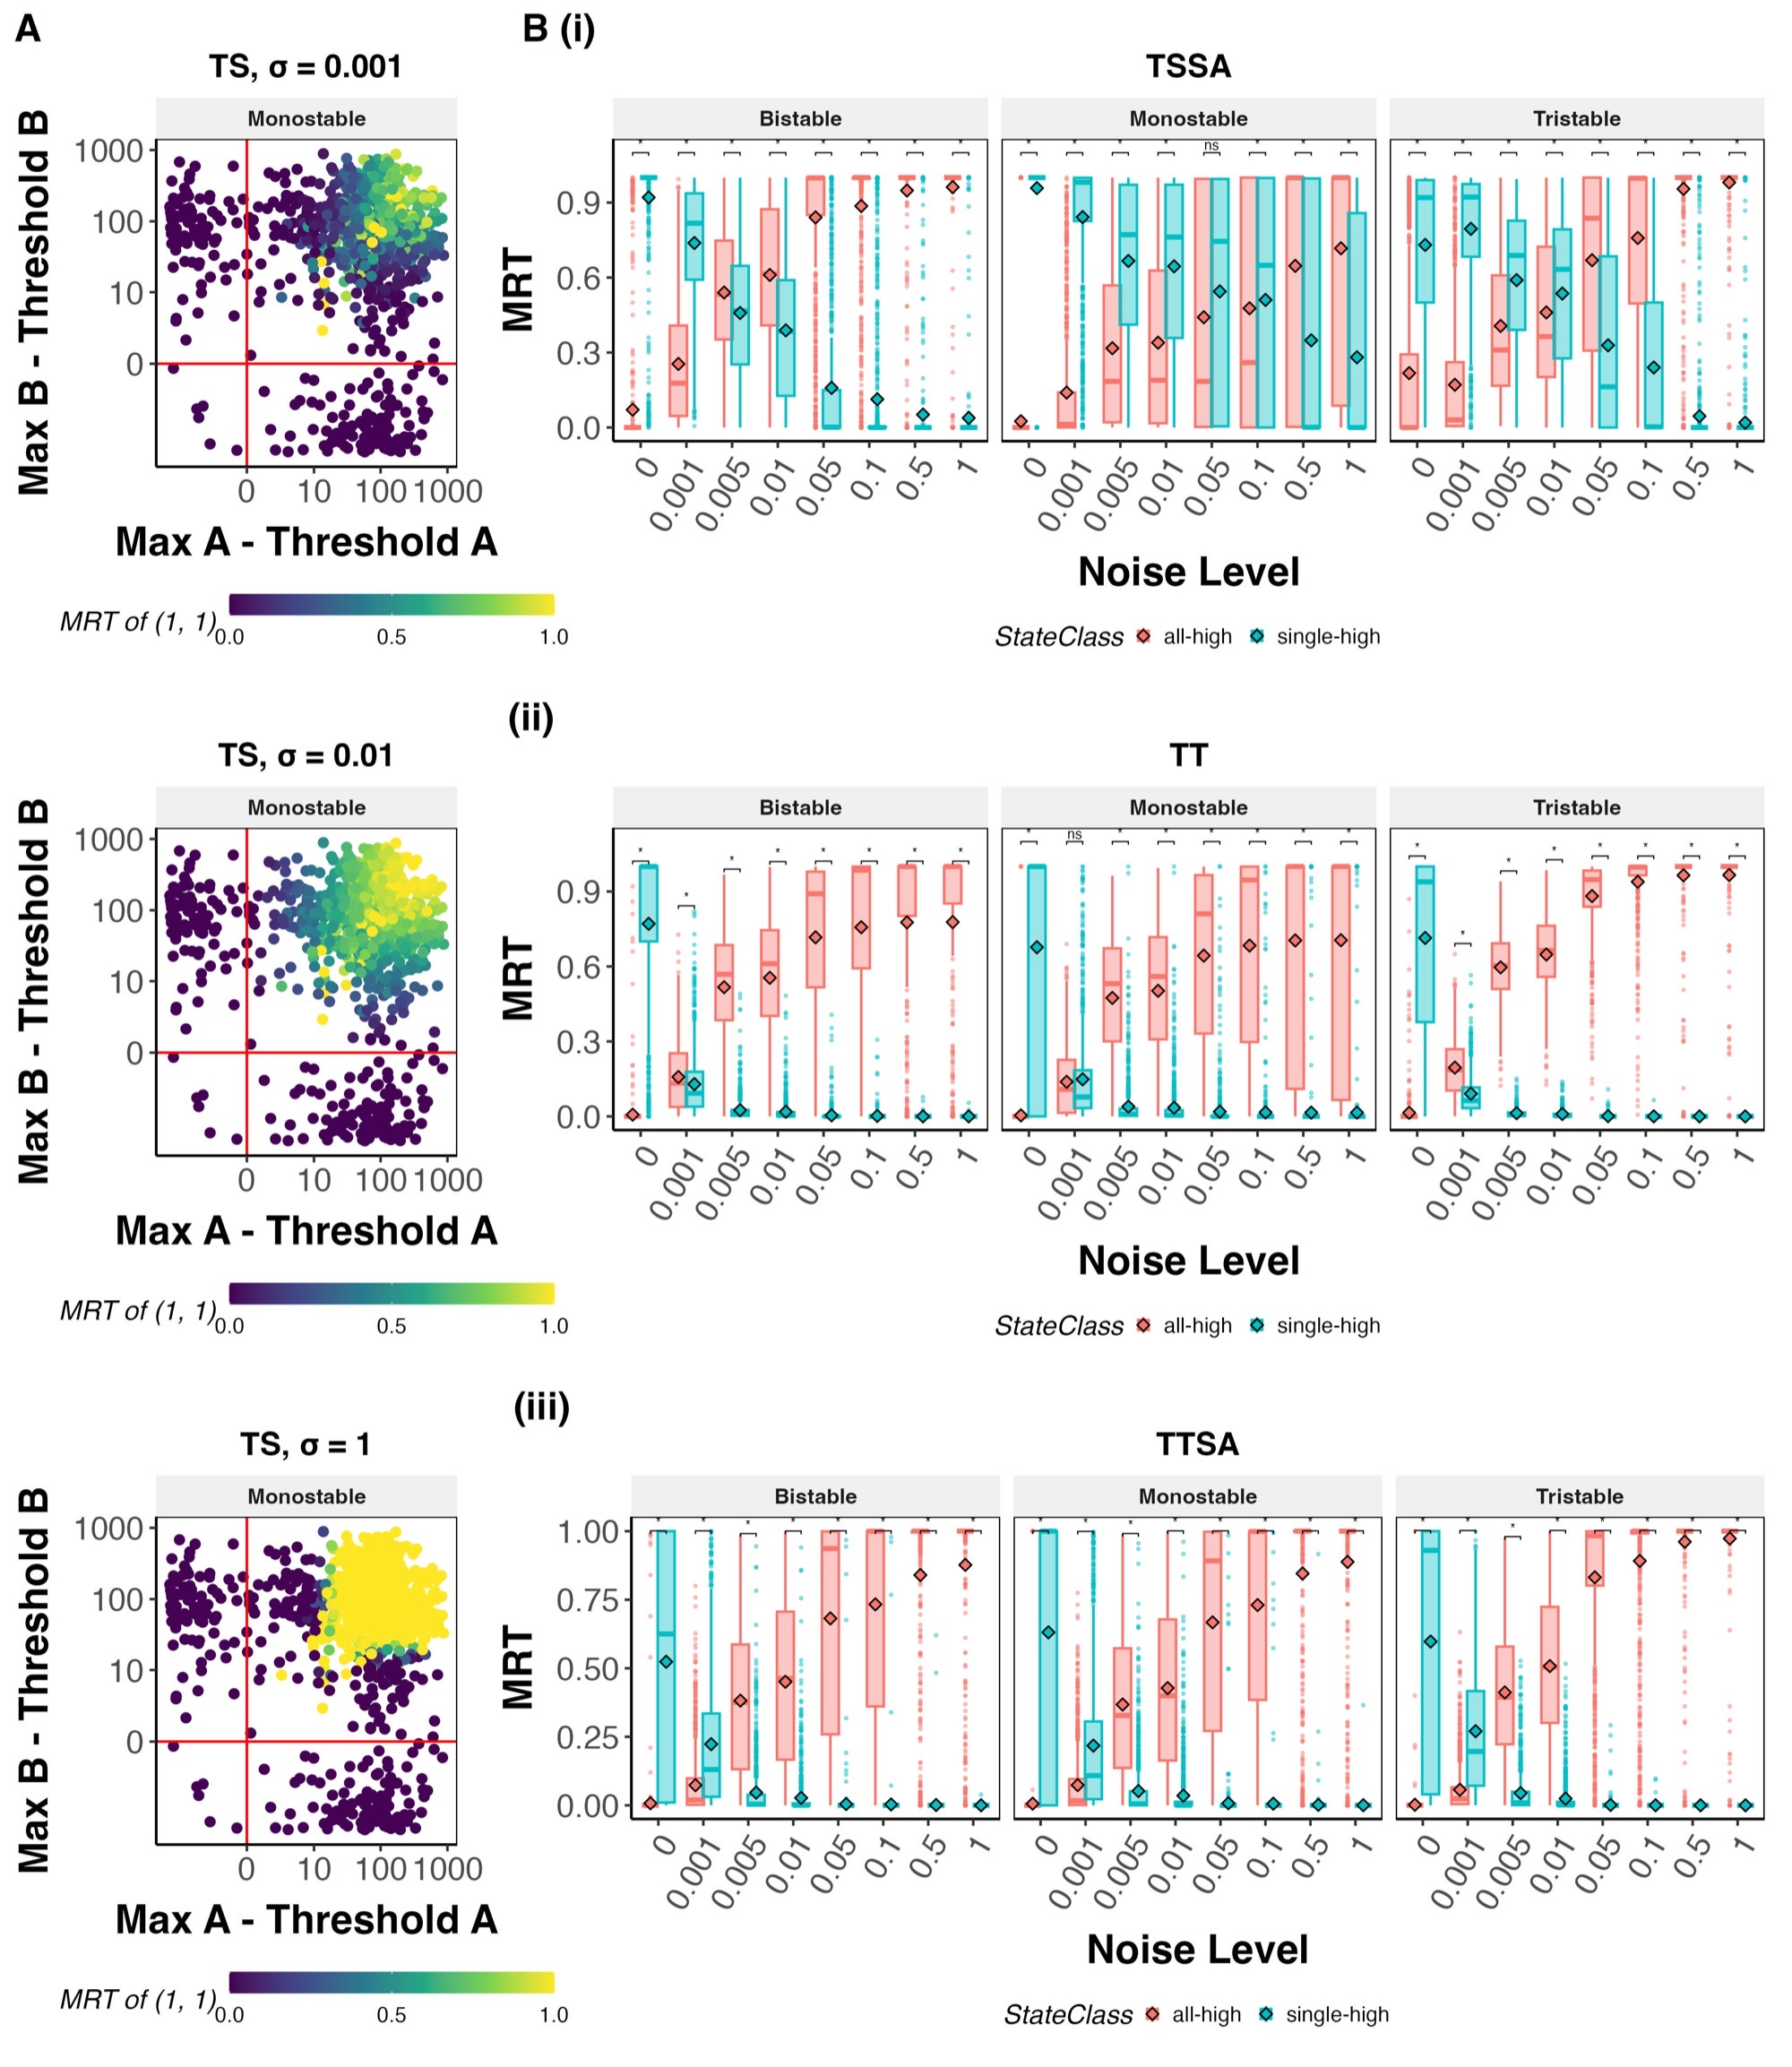
\includegraphics[width=0.8\linewidth]{Fig3S1.jpg}
    \caption{\textbf{(A)} MRT boxplots (as in Fig.\ 3B) for TSSA, TT, and TTSA, stacked vertically. \textbf{(B)} Reachability scatter (as in Figure~\ref{fig:3}C) for the TS network at $\sigma = 0.001, 0.01, 1.0$ (the noise levels not shown in the main figure), stacked vertically. \textbf{(C)} Reachability scatter for the TSSA network at $\sigma = 0.001, 0.01, 0.1, 1.0$.}
    \label{fig:3S1}
\end{figure}

\begin{figure}
    \centering
    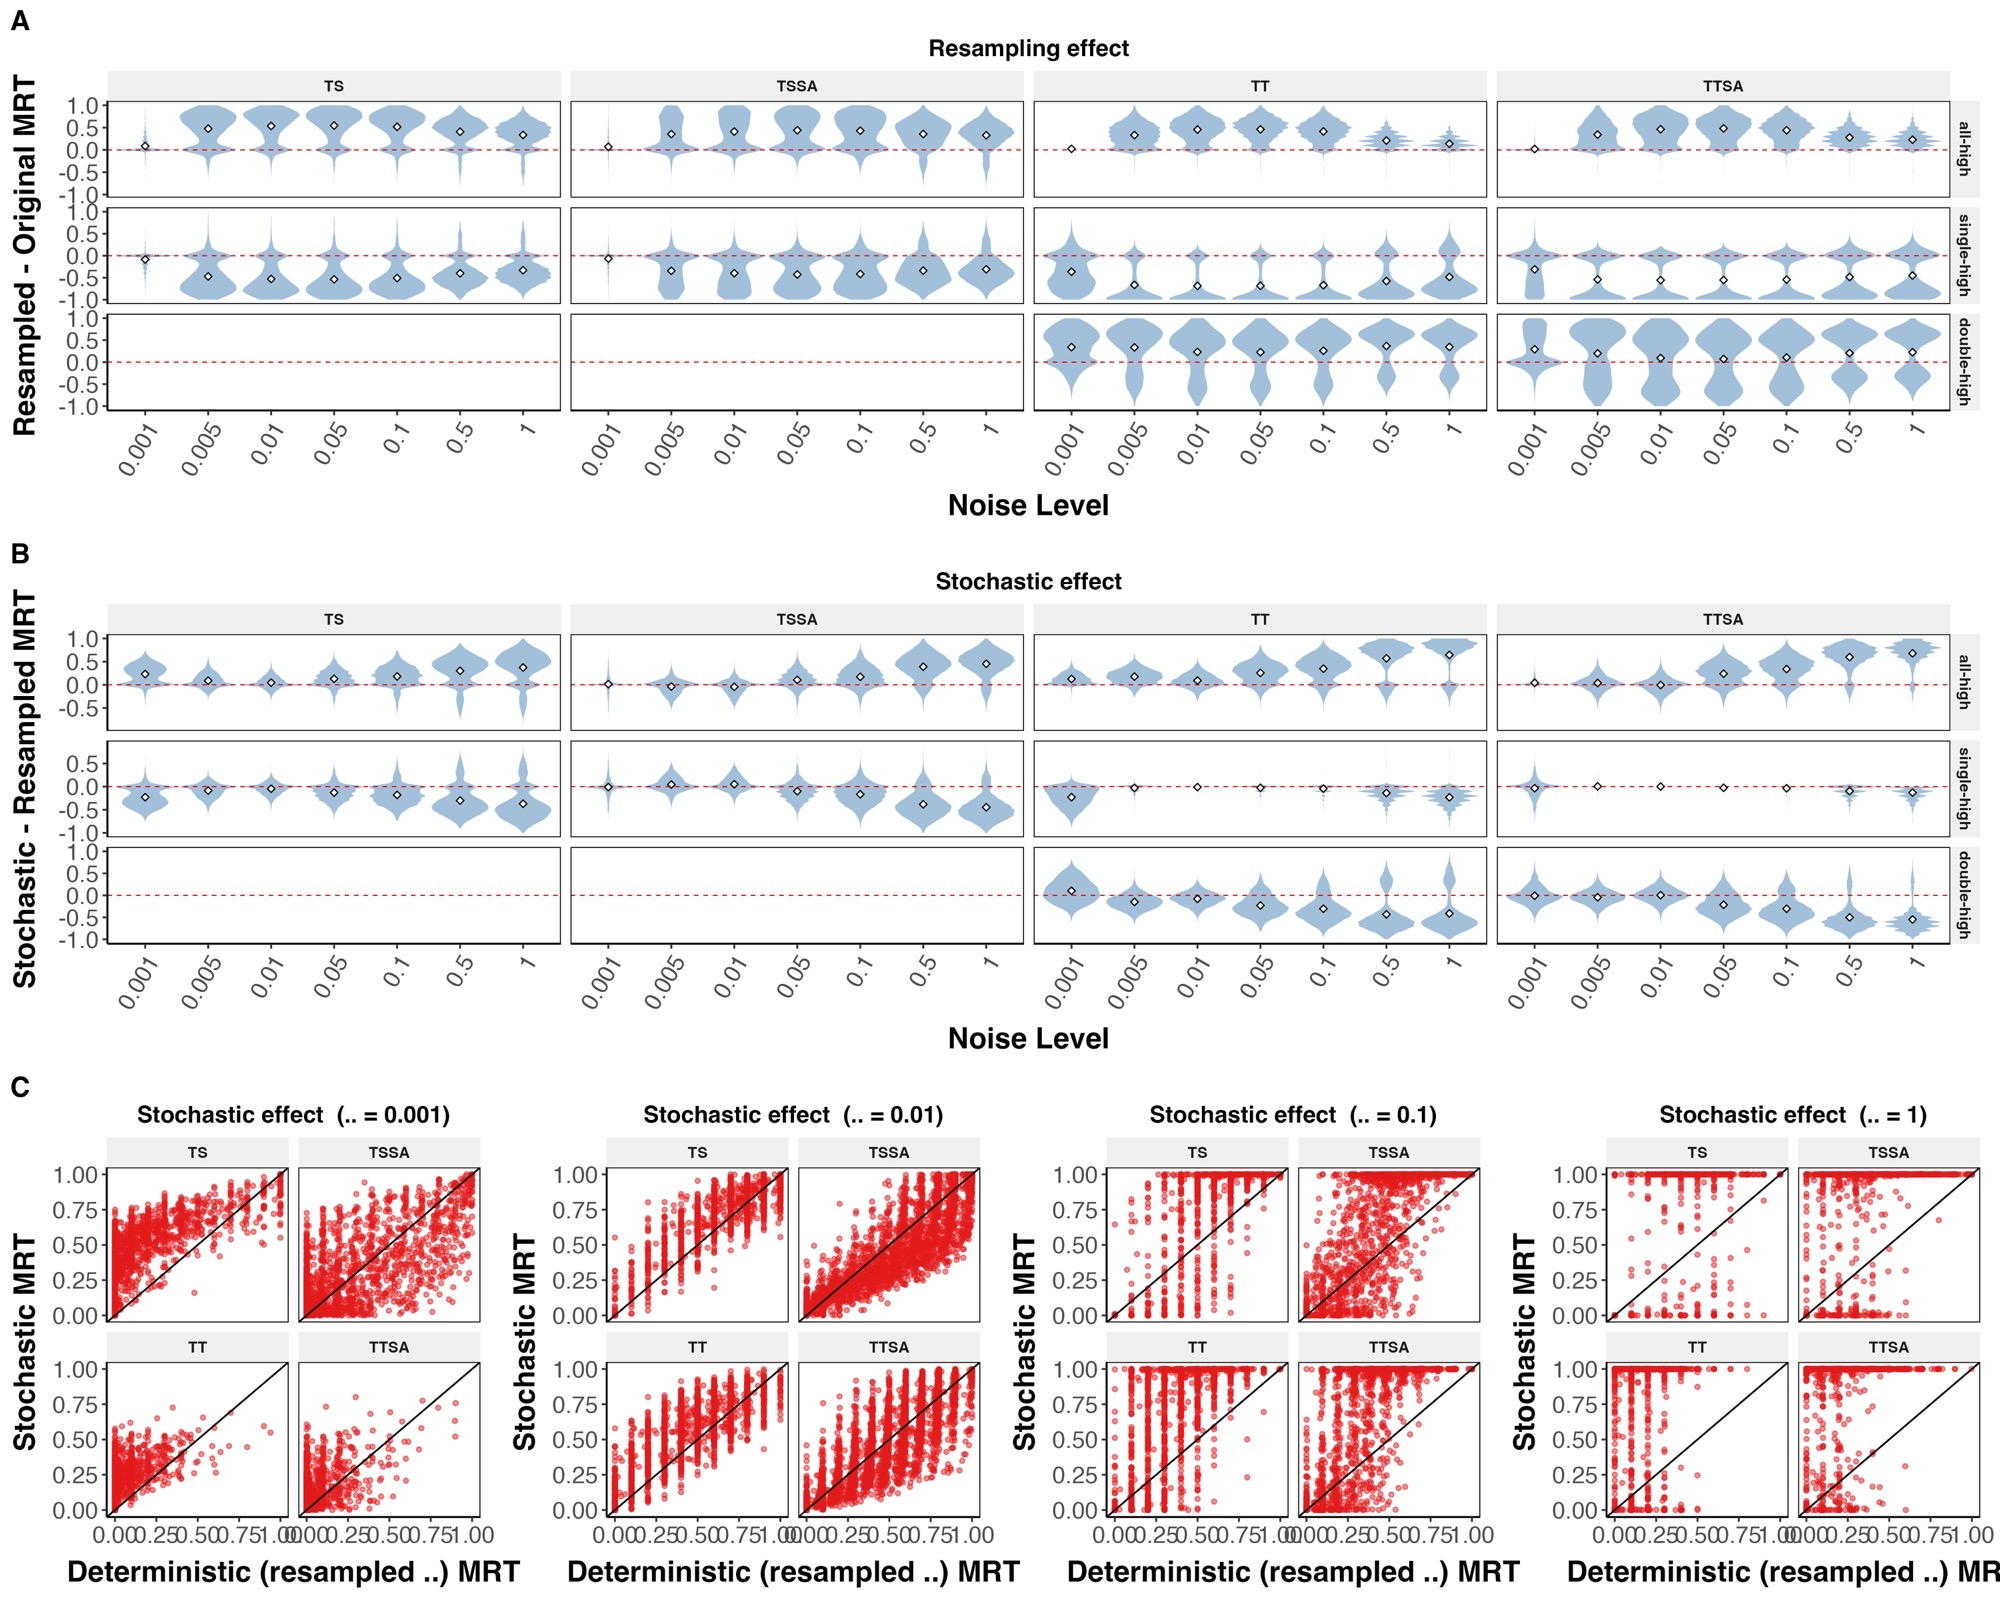
\includegraphics[width=0.8\linewidth]{Fig4S1.jpg}
    \caption{\textbf{(A)} Resampling effect (as in Figure~\ref{fig:3b}B), collapsed to a single per-parameter-set difference and shown across all noise levels, faceted by state class (all-high/single-high/double-high) and network (TS, TSSA, TT, TTSA). \textbf{(B)} Same, for the stochastic effect. \textbf{(C)} Paramwise scatter of resampled-$\lambda$ deterministic vs.\ stochastic MRT of the all-high state, all four networks, at each of four noise levels (0.001, 0.01, 0.1, 1.0).}
    \label{fig:3bS1}
\end{figure}

\begin{figure}
    \centering
    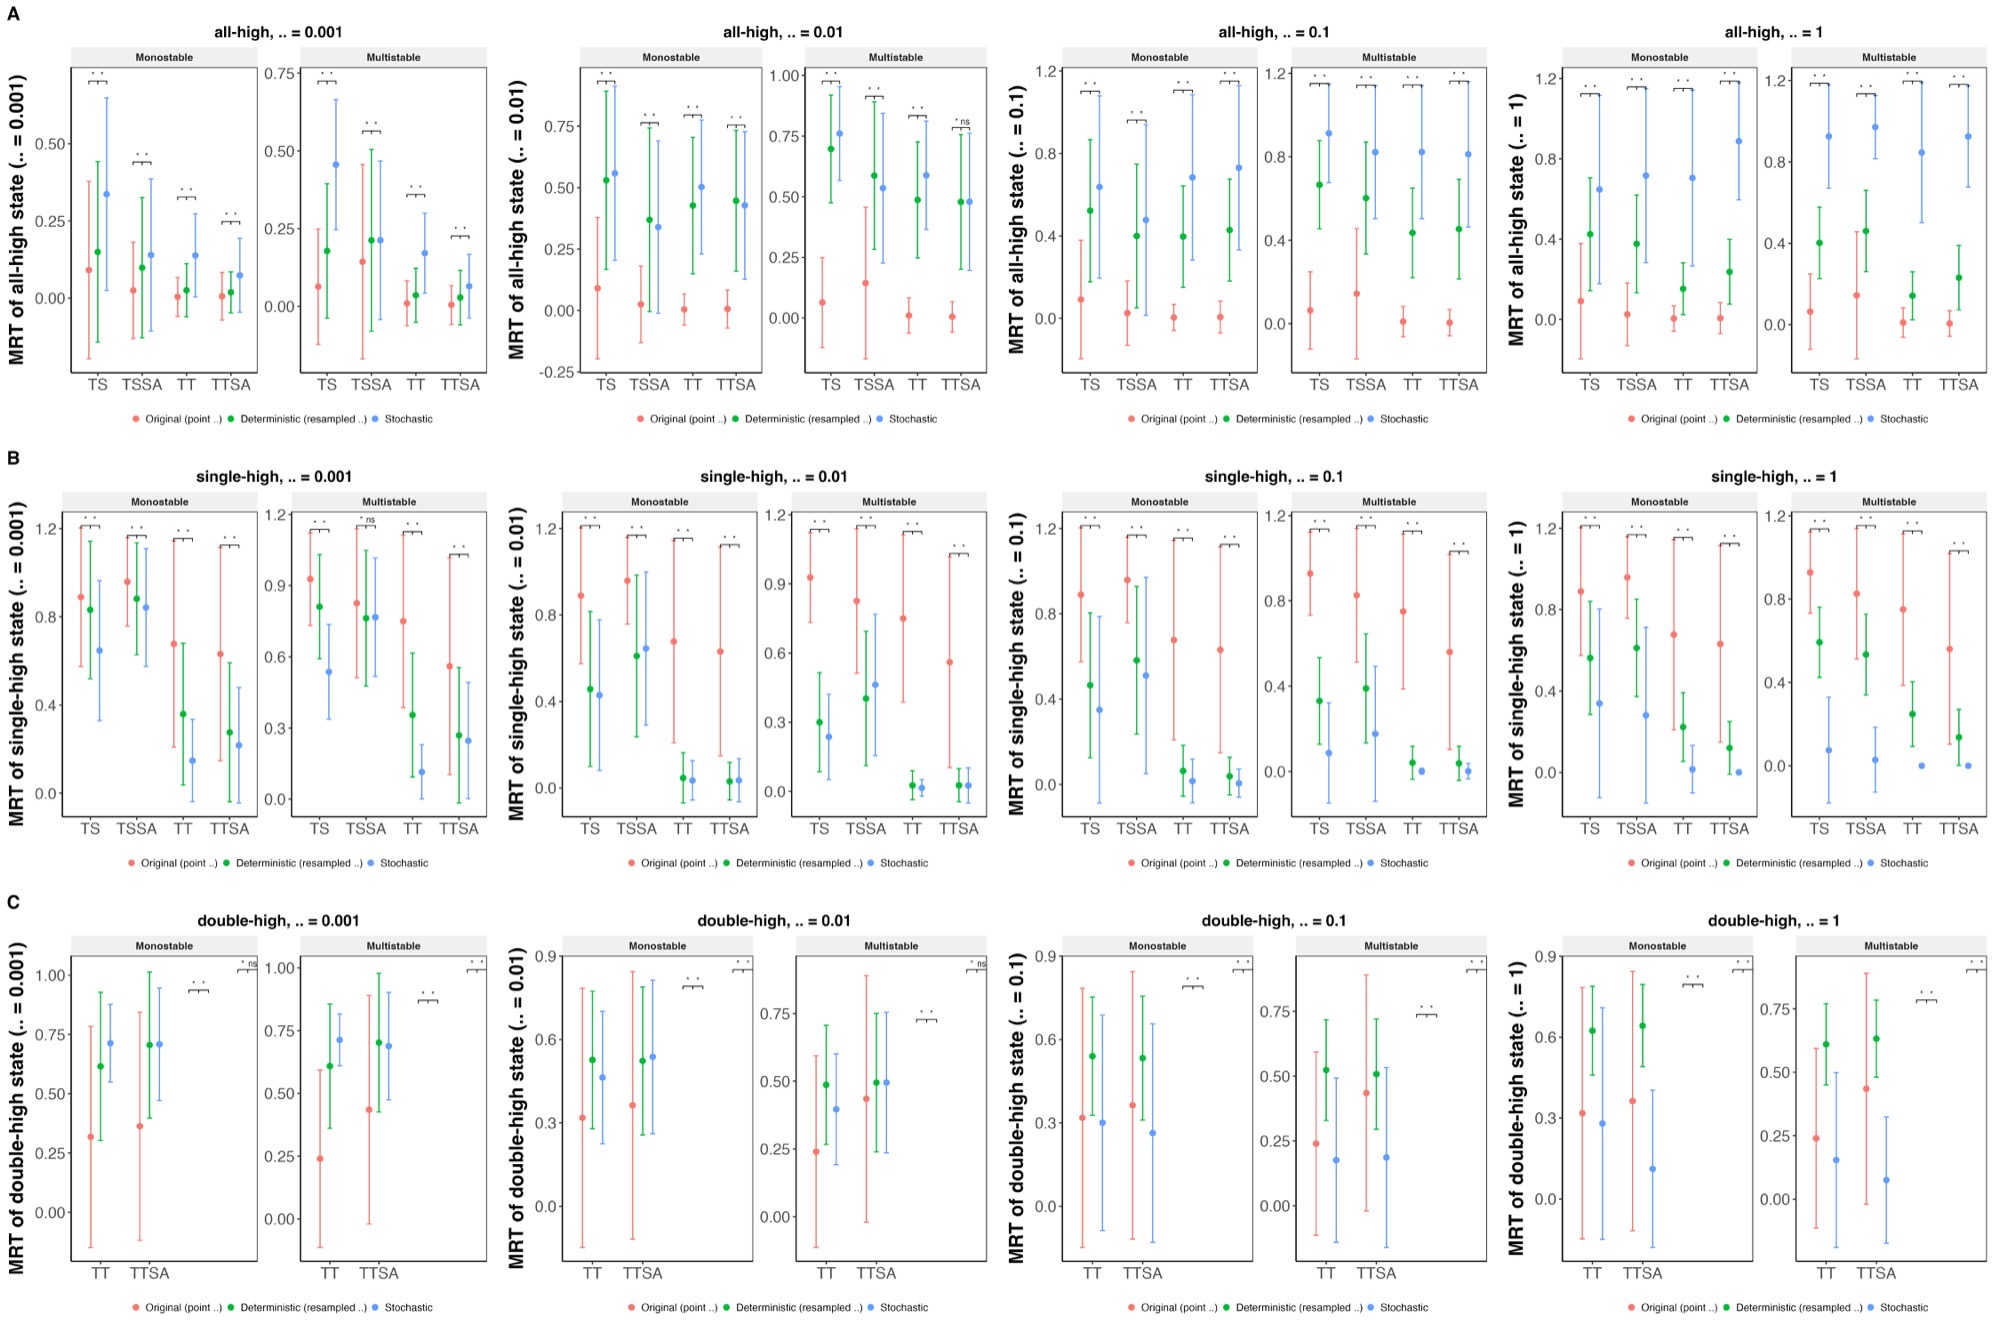
\includegraphics[width=0.8\linewidth]{Fig4S2.jpg}
    \caption{All-high \textbf{(A)}, single-high \textbf{(B)}, and double-high \textbf{(C)} state MRT comparisons (as in Figure~\ref{fig:3b}D: original/resampled/stochastic, faceted by stability class), repeated at four noise levels (columns: 0.001, 0.01, 0.1, 1.0), for TS, TSSA, TT, TTSA. 2-node networks (TS, TSSA) have no double-high state distinct from all-high, so they are absent from that row.
}
    \label{fig:3bS2}
\end{figure}

\begin{figure}
    \centering
    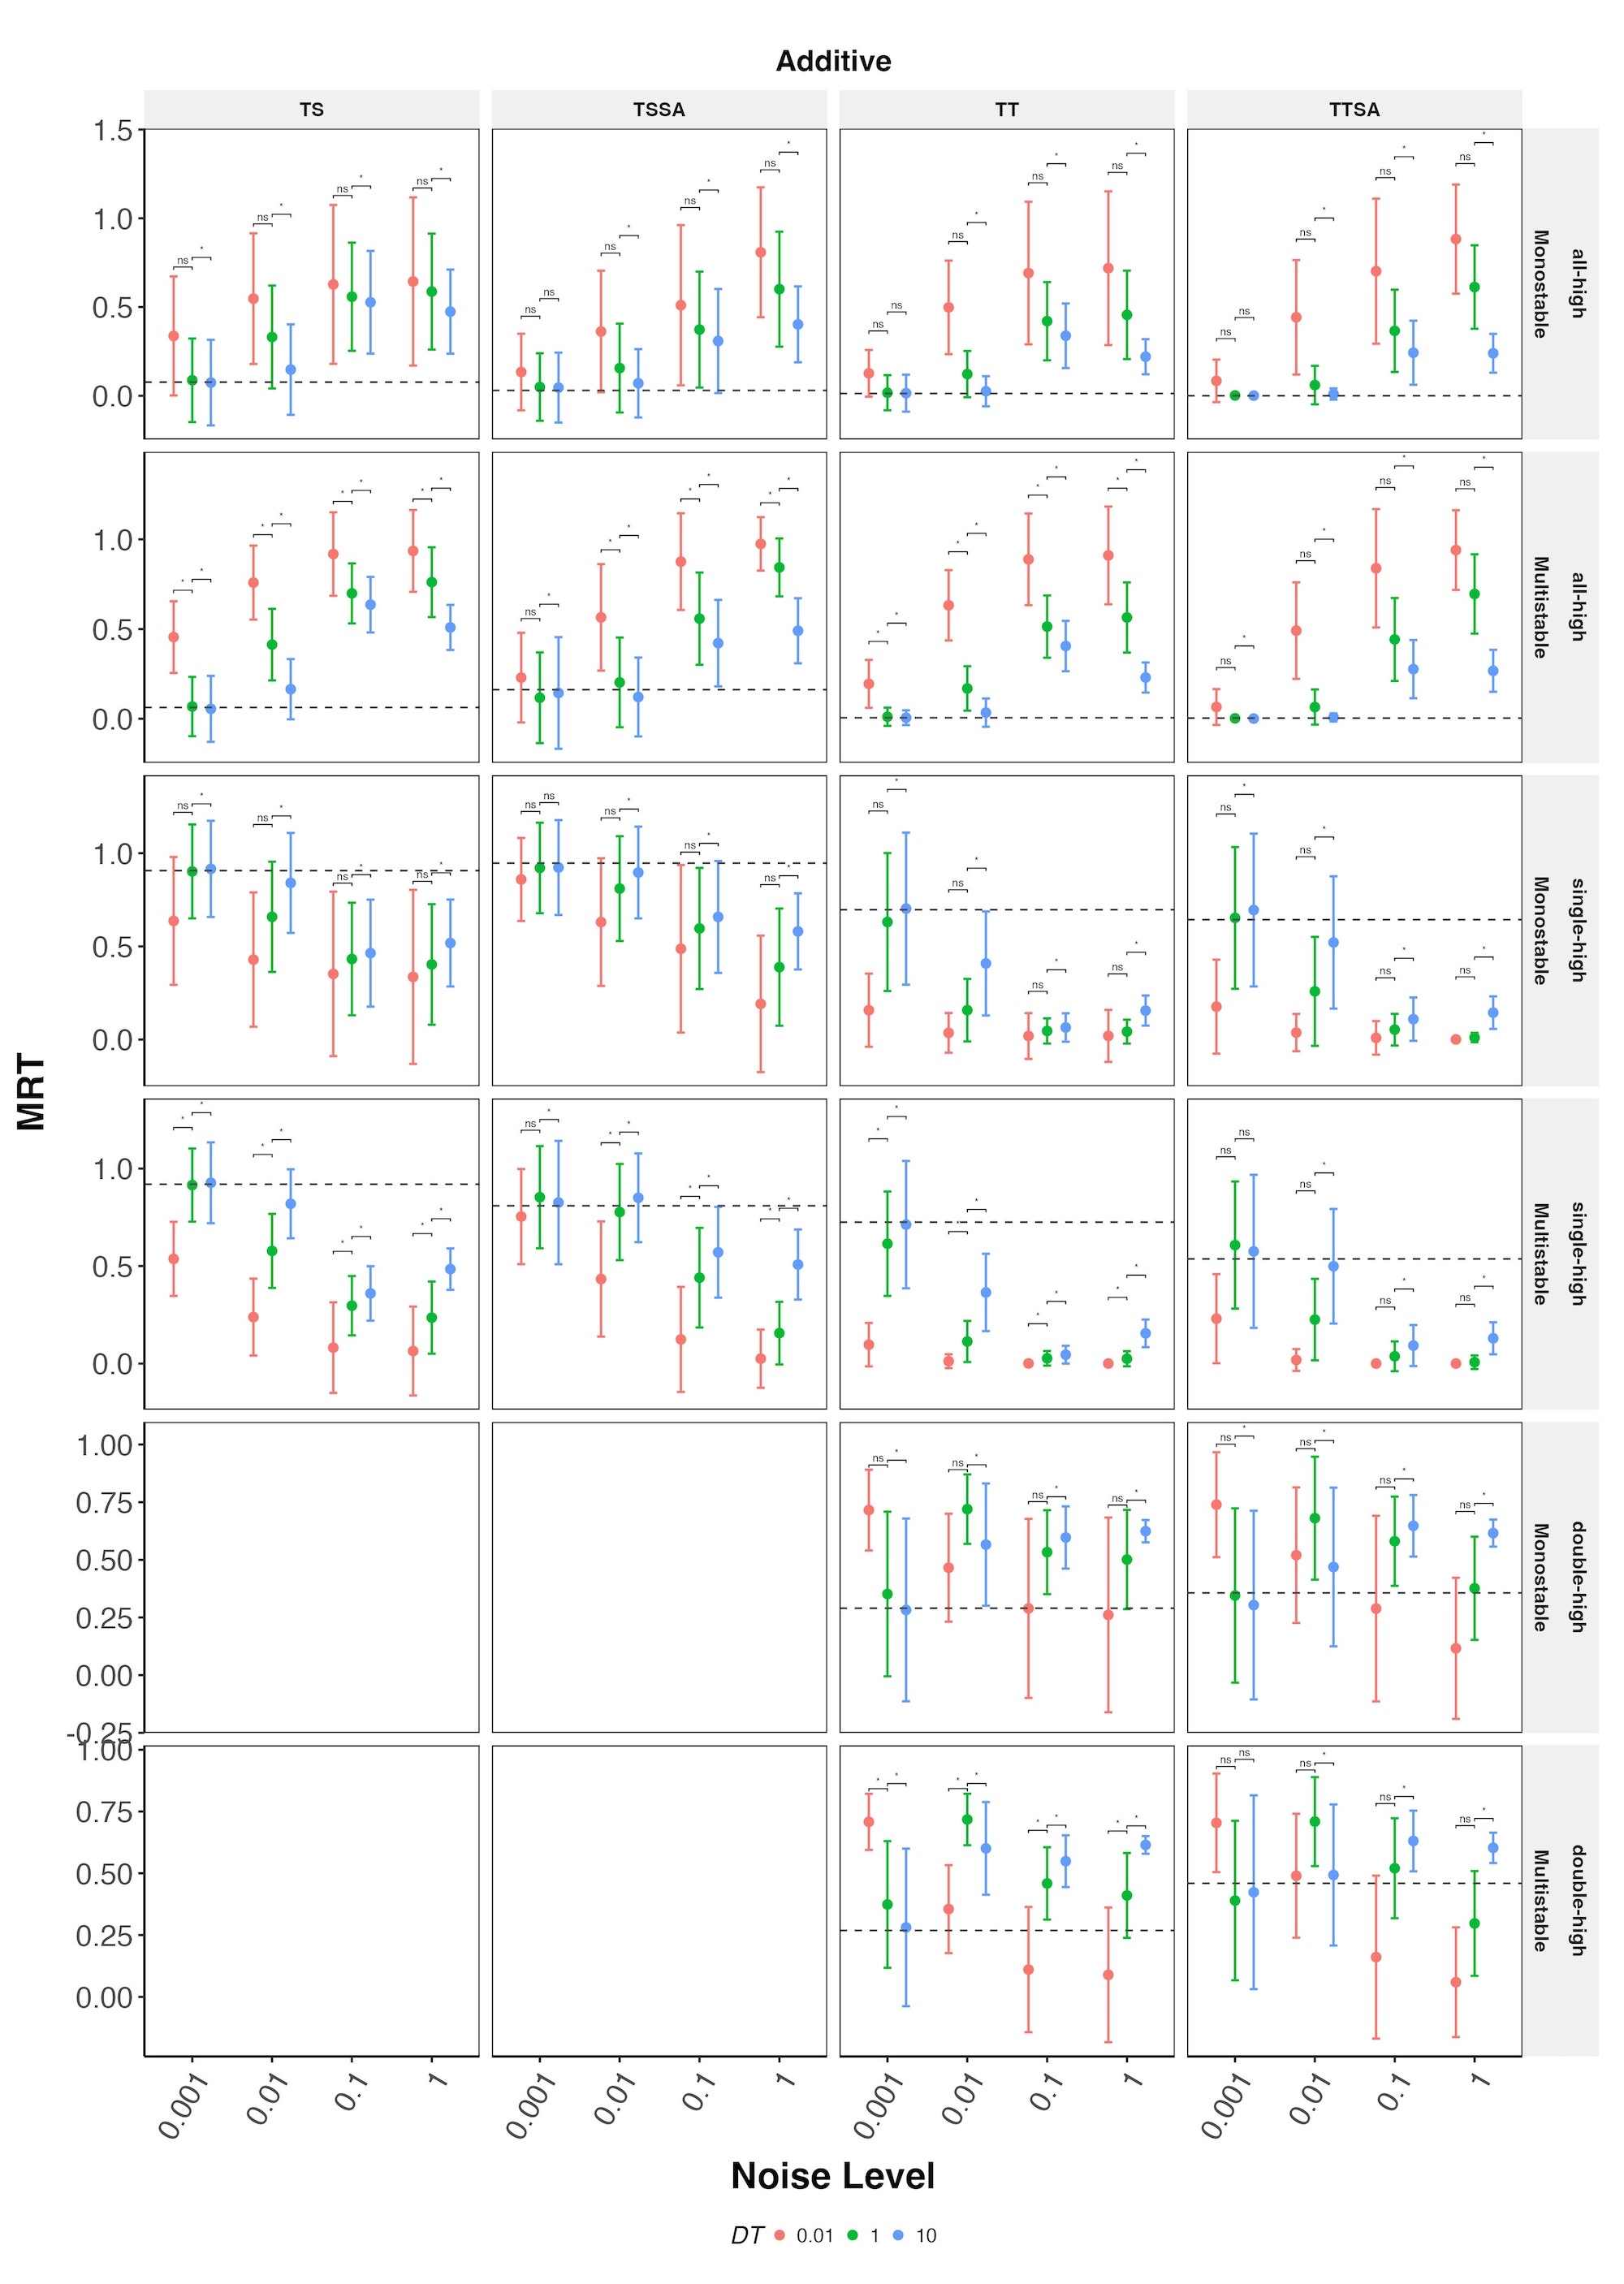
\includegraphics[width=0.8\linewidth]{Fig4S3.jpg}
    \caption{Comparison of MRTs for additive noise simulated at different values of $dt$}
    \label{fig:3bS3}
\end{figure}


\begin{figure}
    \centering
    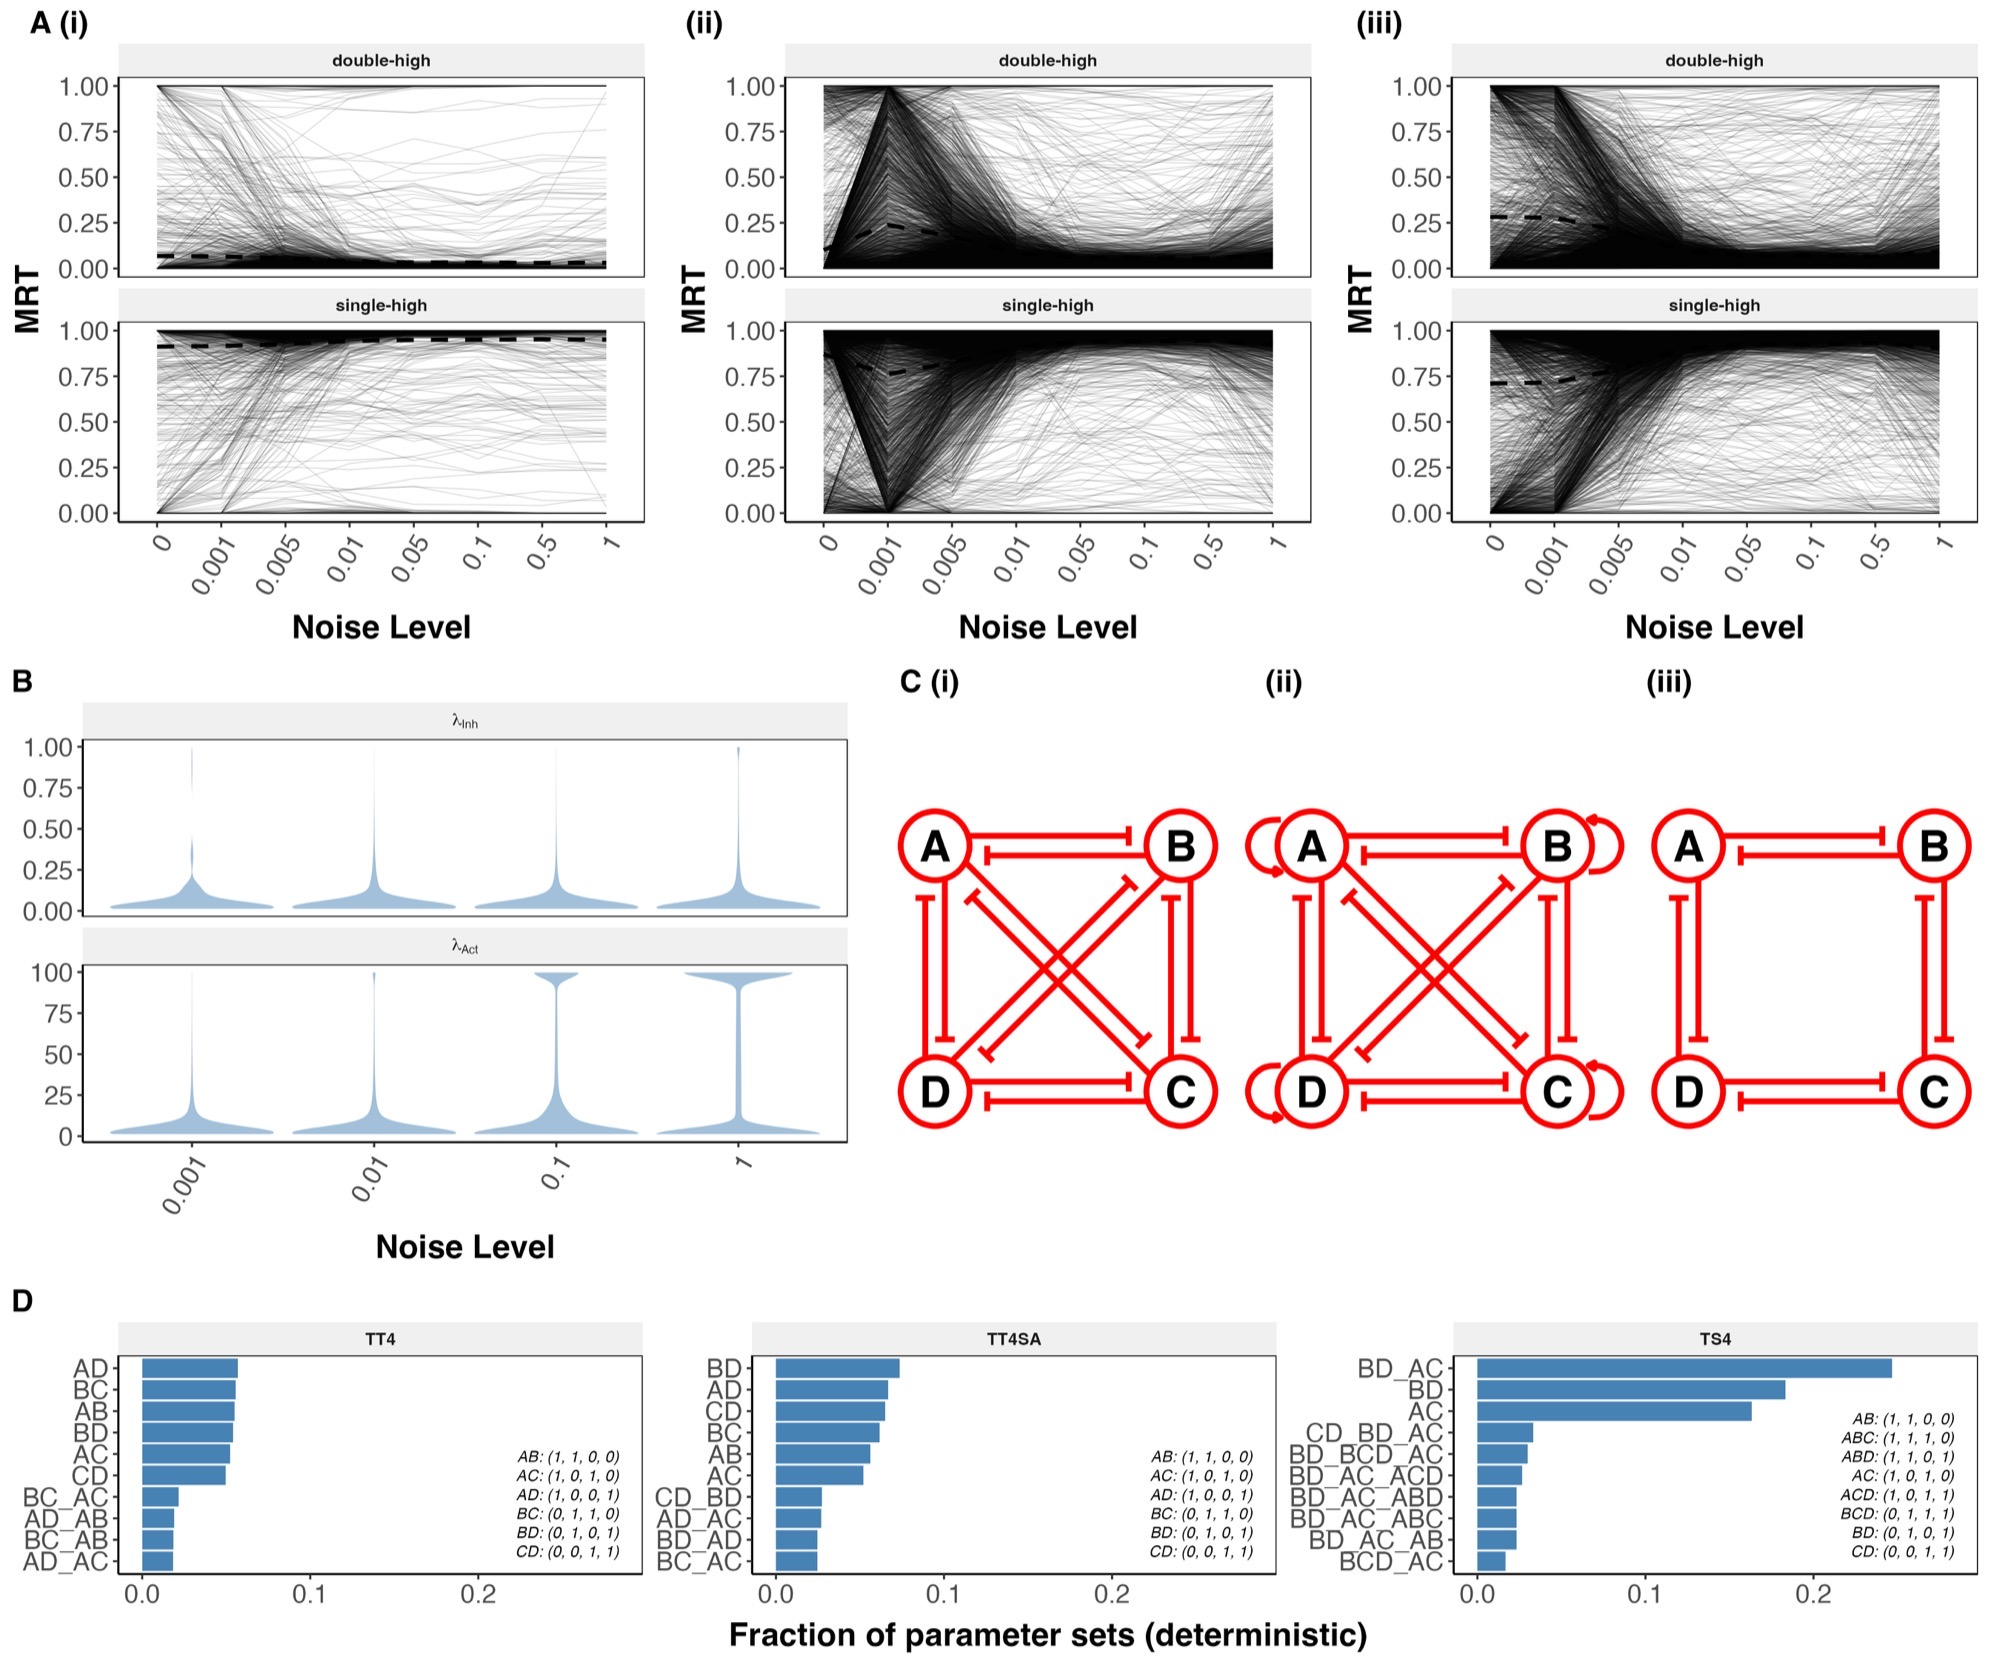
\includegraphics[width=0.8\linewidth]{Fig5S1.jpg}
    \caption{\textbf{(A)} MRT vs.\ noise level (as in Figure~\ref{fig:4}A, each showing a random sample of 100 parameter-set trajectories with the mean across the full population) for TS, TSSA, and TT; single-high and double-high state classes. For TS and TSSA, whose fully-active state is intrinsically ``all-high'' rather than a distinct ``double-high'' state, this facet is relabeled ``double-high'' for consistency with the other panels, but shows the same all-high data. \textbf{(B)} $\lambda$ distributions (as in Figure~\ref{fig:3b}A) under Multiplicative noise. \textbf{(C)} Network topology diagrams for TT4, TT4SA, and TS4. \textbf{(D)} Deterministic attractor-combination frequency (as in Fig.\ 1C, but from the noise-simulation pipeline's zero-noise runs rather than RACIPE's own steady-state search) for TT4, TT4SA, and TS4.
}
    \label{fig:4S1}
\end{figure}

\begin{figure}
    \centering
    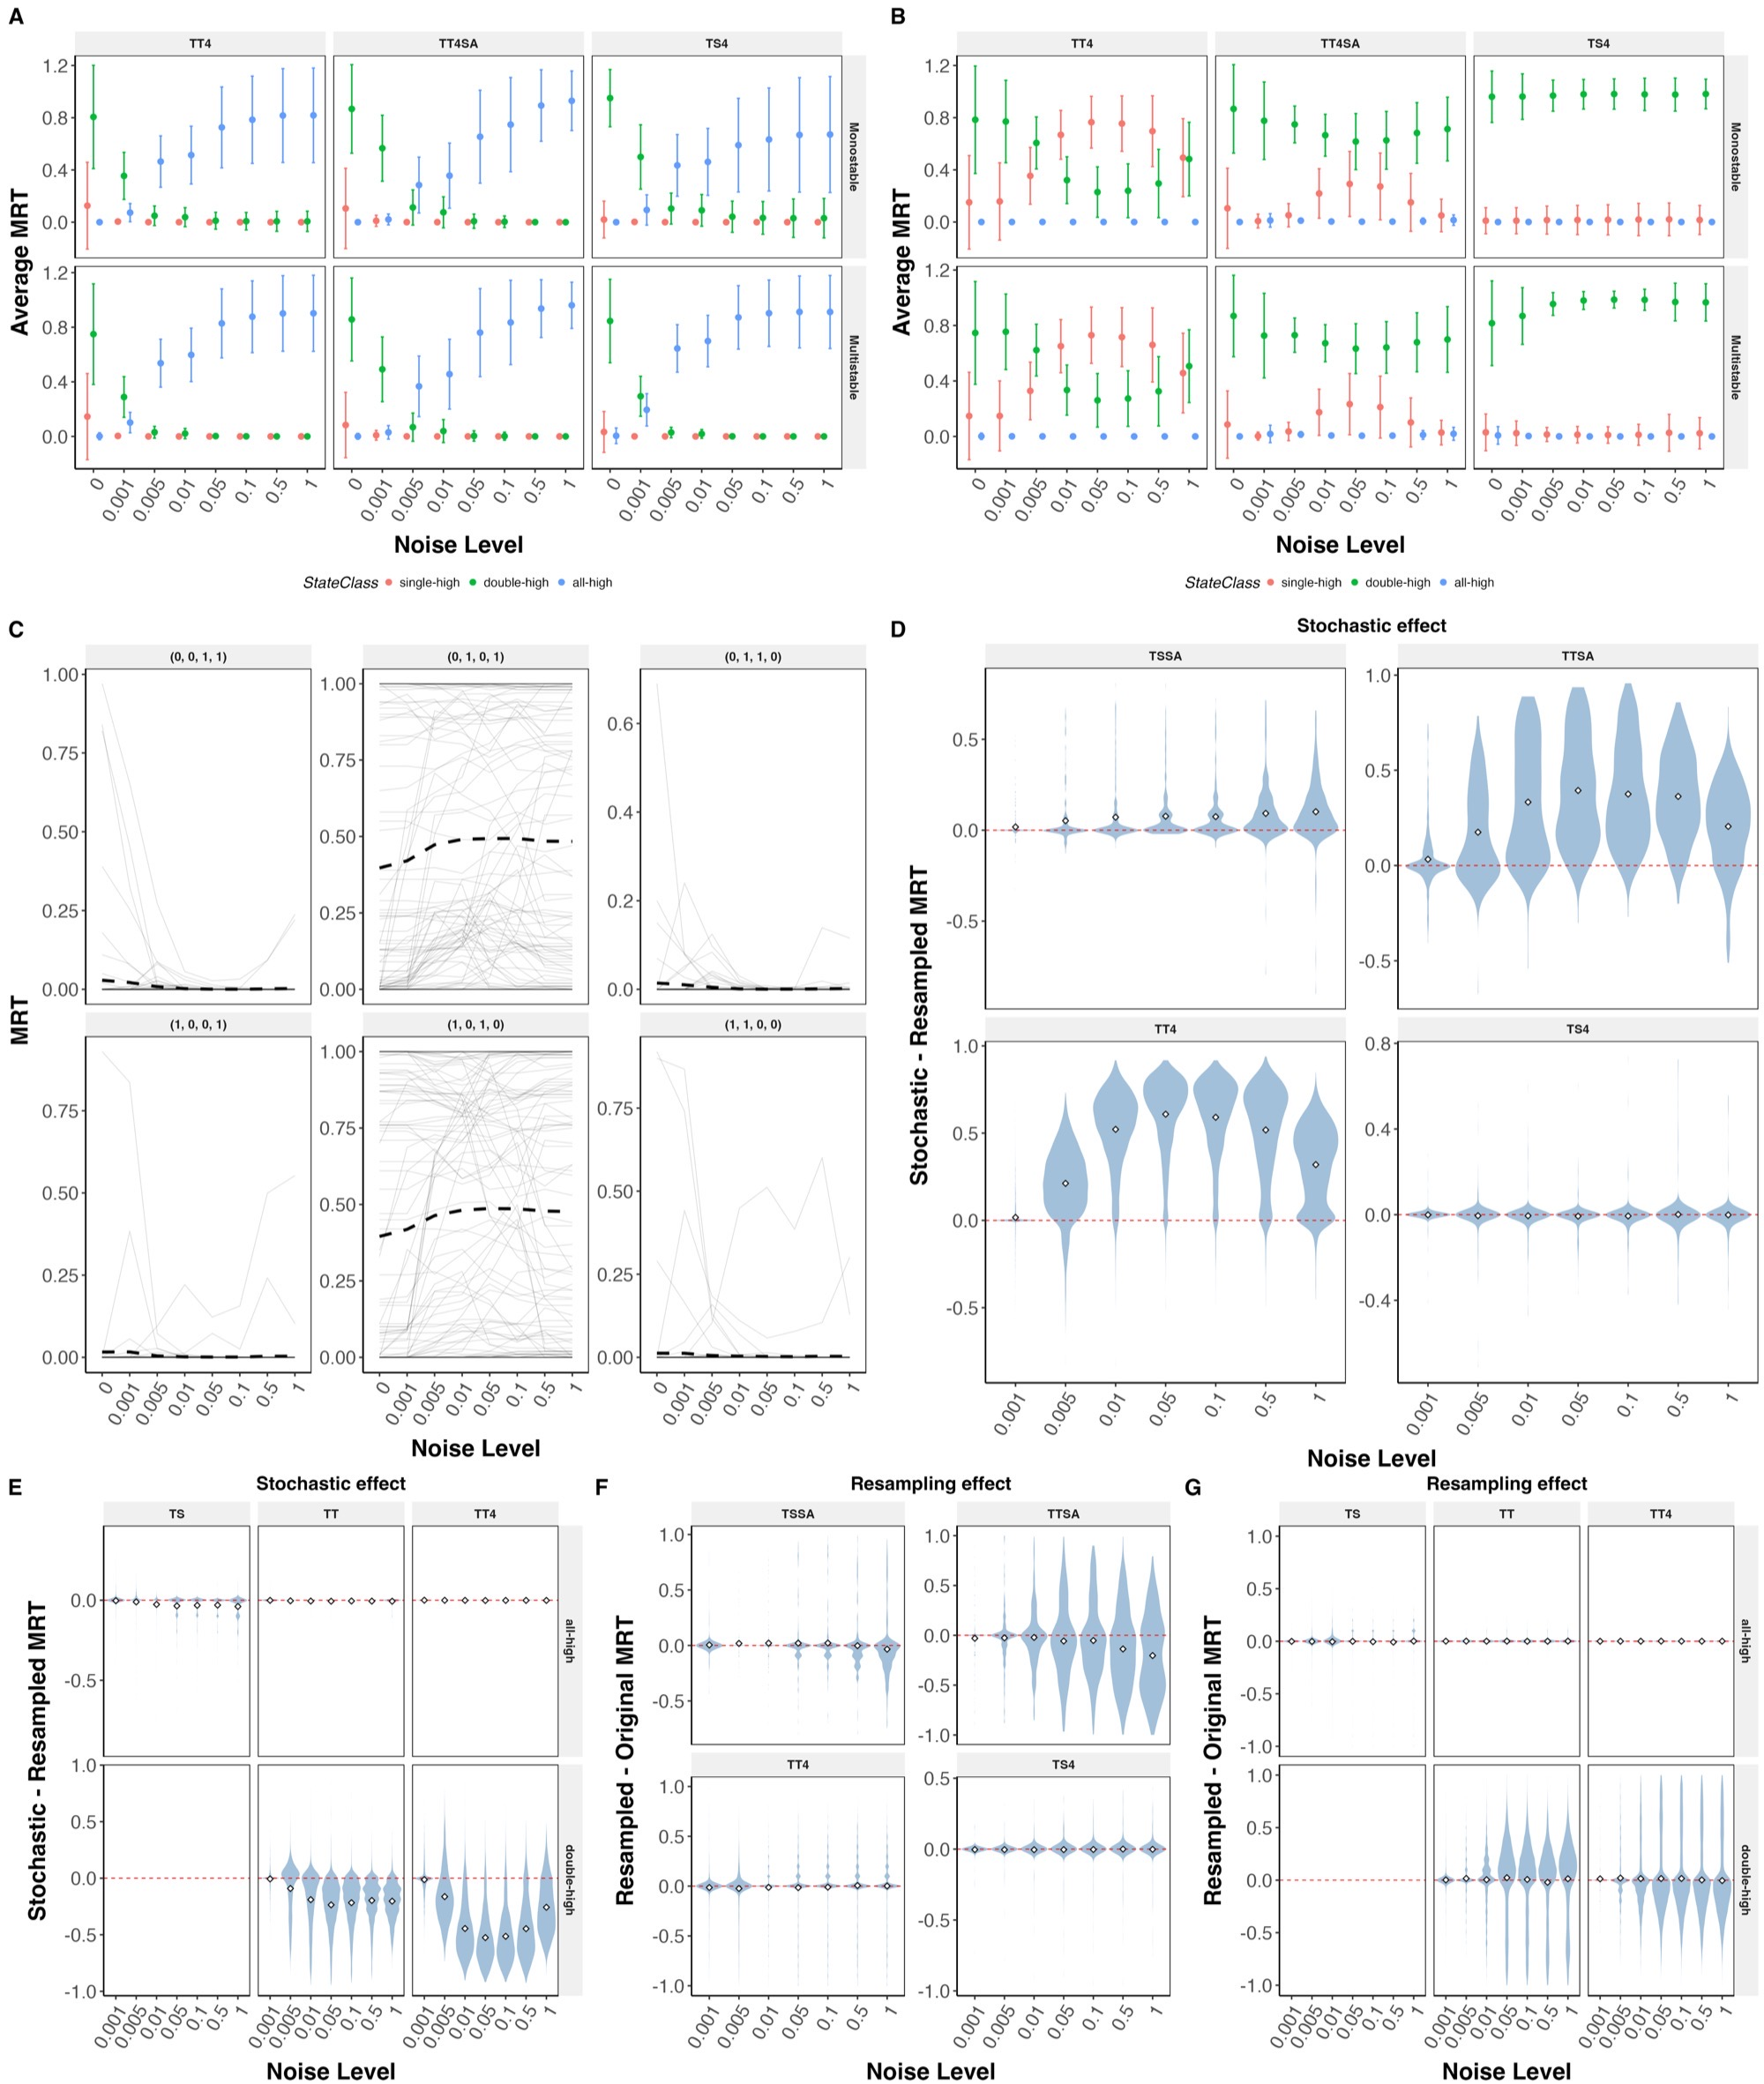
\includegraphics[width=0.8\linewidth]{Fig5S2.jpg}
    \caption{\textbf{(A, B)} MRT vs.\ noise level for TT4, TT4SA, and TS4; single-high, double-high, and all-high states, faceted by stability class, under Additive (A) and Multiplicative (B) noise. \textbf{(C)} State-wise MRT vs.\ noise level for each of TS4's six double-high states individually (Multiplicative noise), showing that the same subset of states dominates at every noise level; grey lines show a random sample of 100 parameter-set trajectories, with the mean across the full parameter population shown separately. \textbf{(D)} Stochastic effect for the single-high state, across noise levels, for TSSA, TTSA, TT4, and TS4. \textbf{(E)} Stochastic effect for the all-high and double-high states, for TS, TT, and TT4. \textbf{(D$'$, E$'$)} Same networks/state classes as D and E, respectively, but showing the resampling effect instead of the stochastic effect.
}
    \label{fig:4S2}
\end{figure}

\begin{figure}
    \centering
    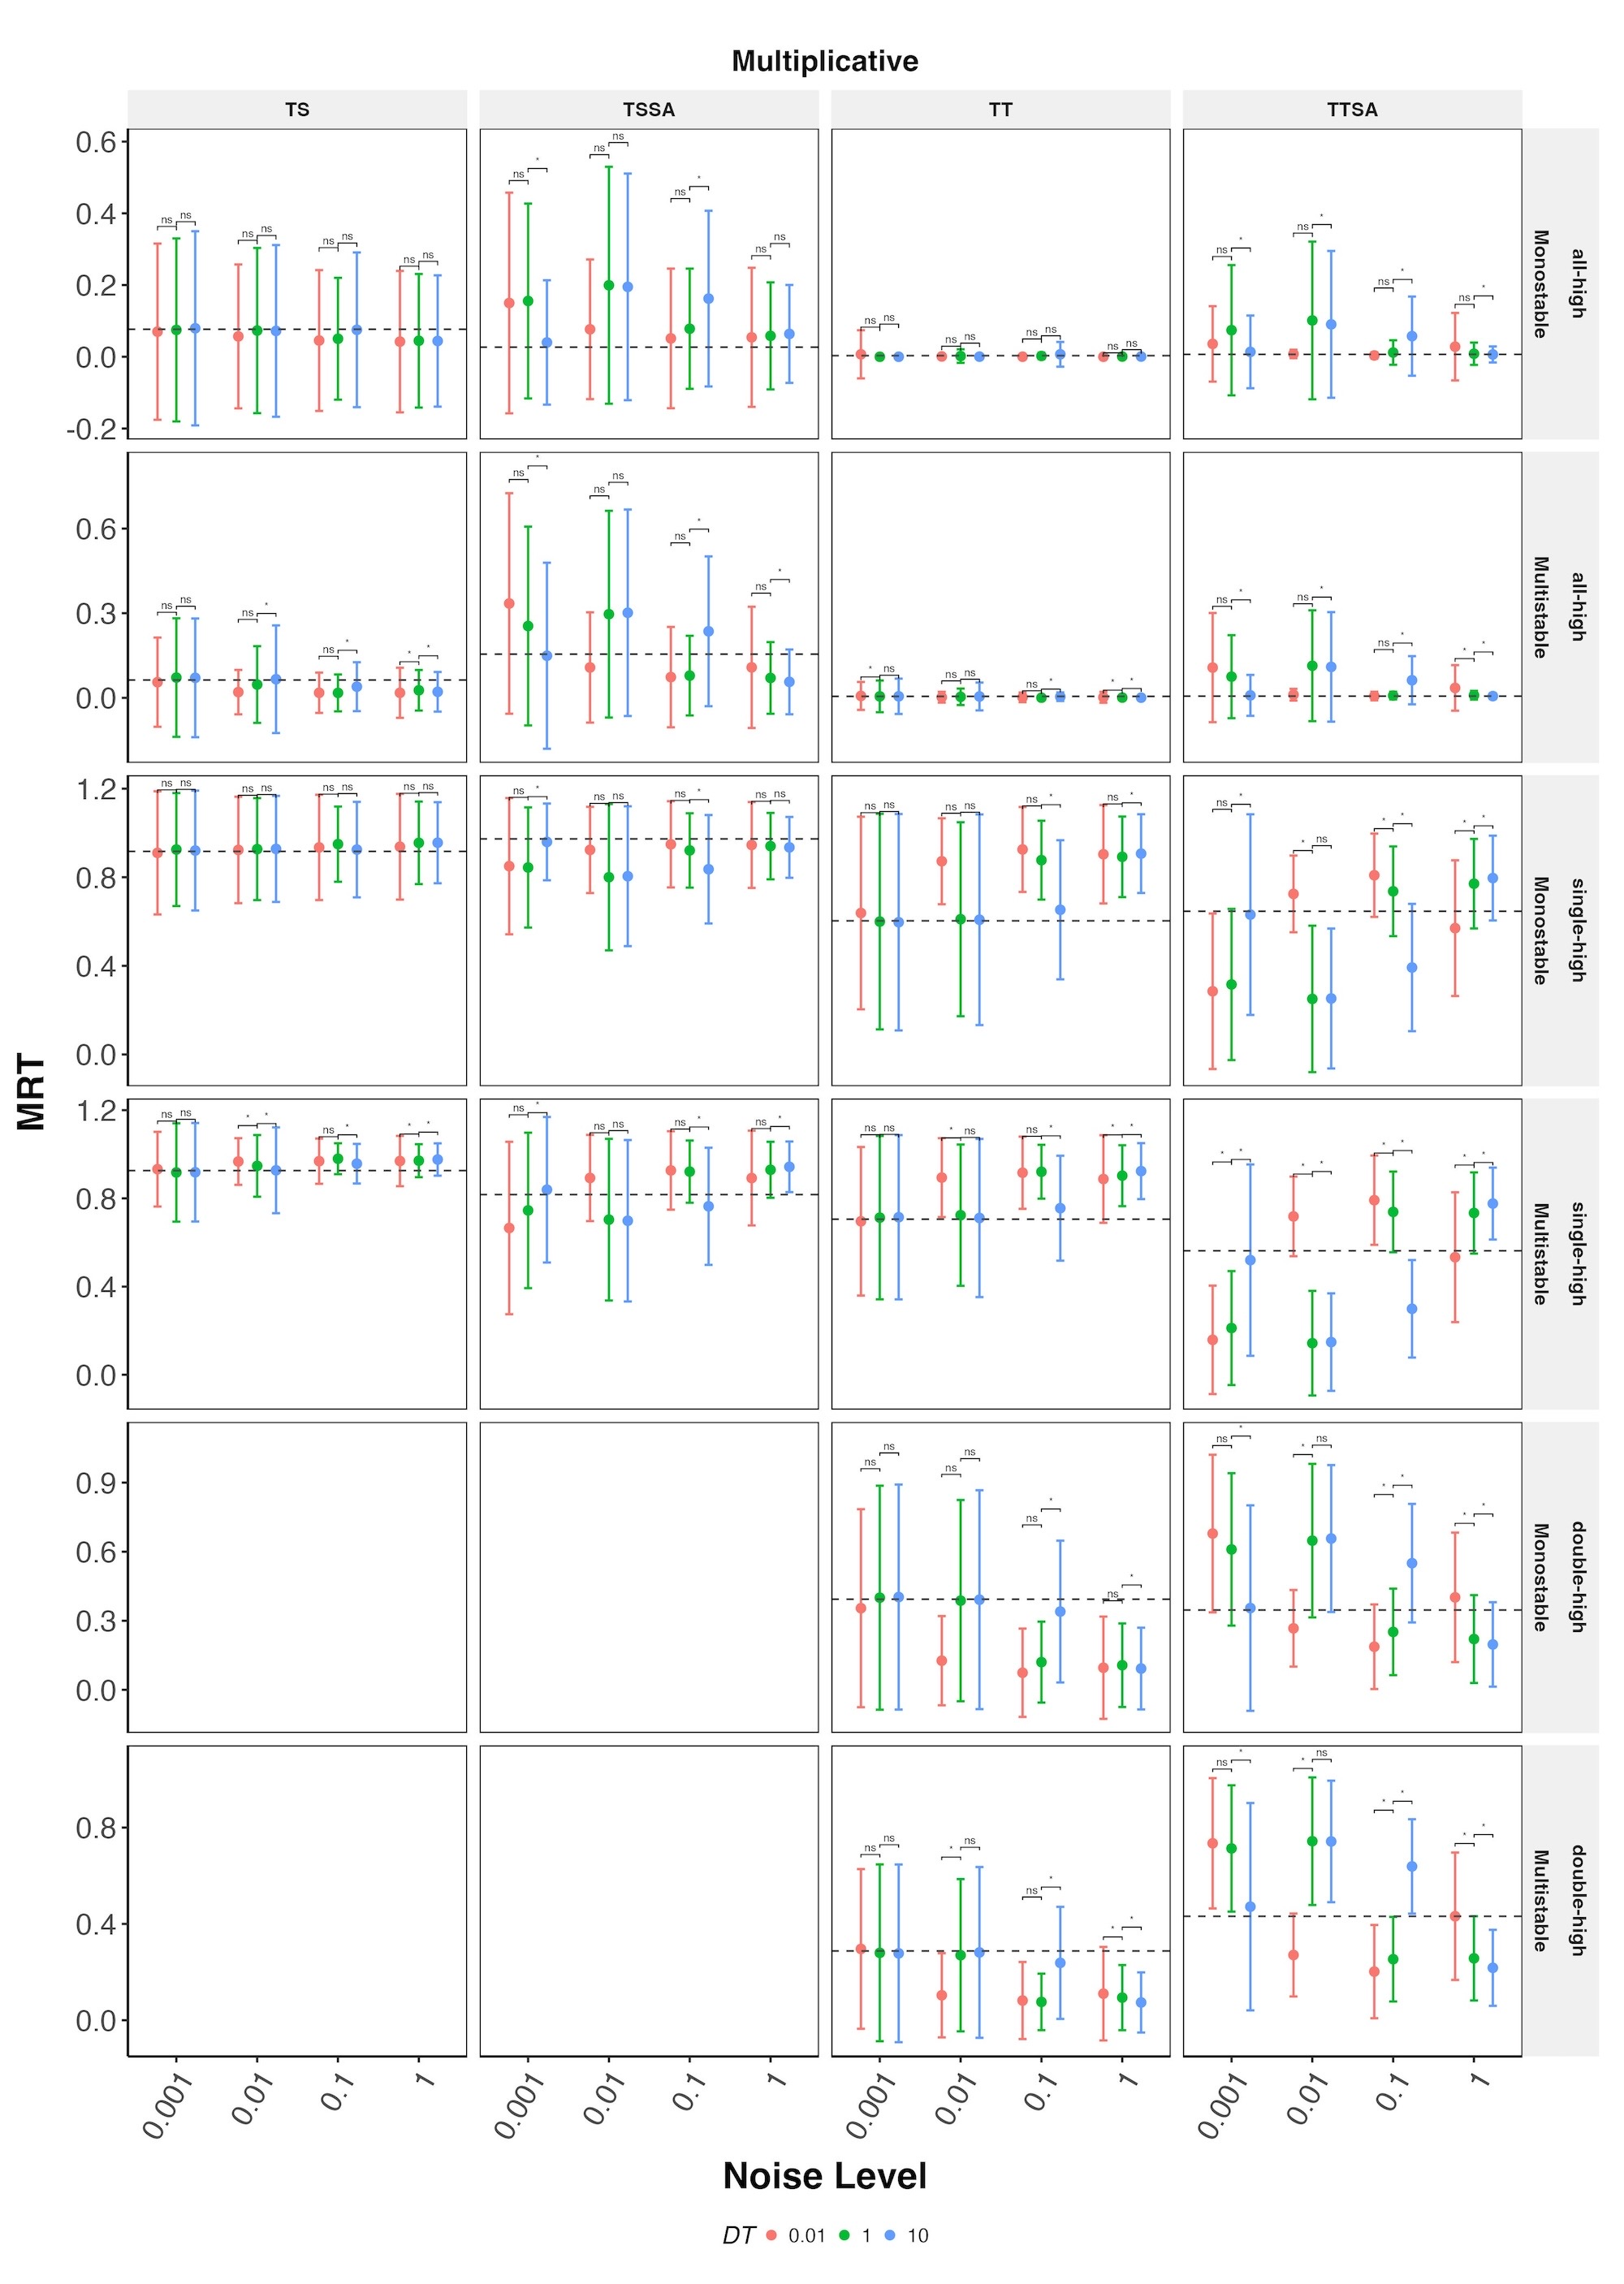
\includegraphics[width=0.8\linewidth]{Fig5S3.jpg}
    \caption{Comparison of MRTs for multiplicative noise simulated at different values of $dt$}
    \label{fig:4S3}
\end{figure}

\begin{figure}
    \centering
    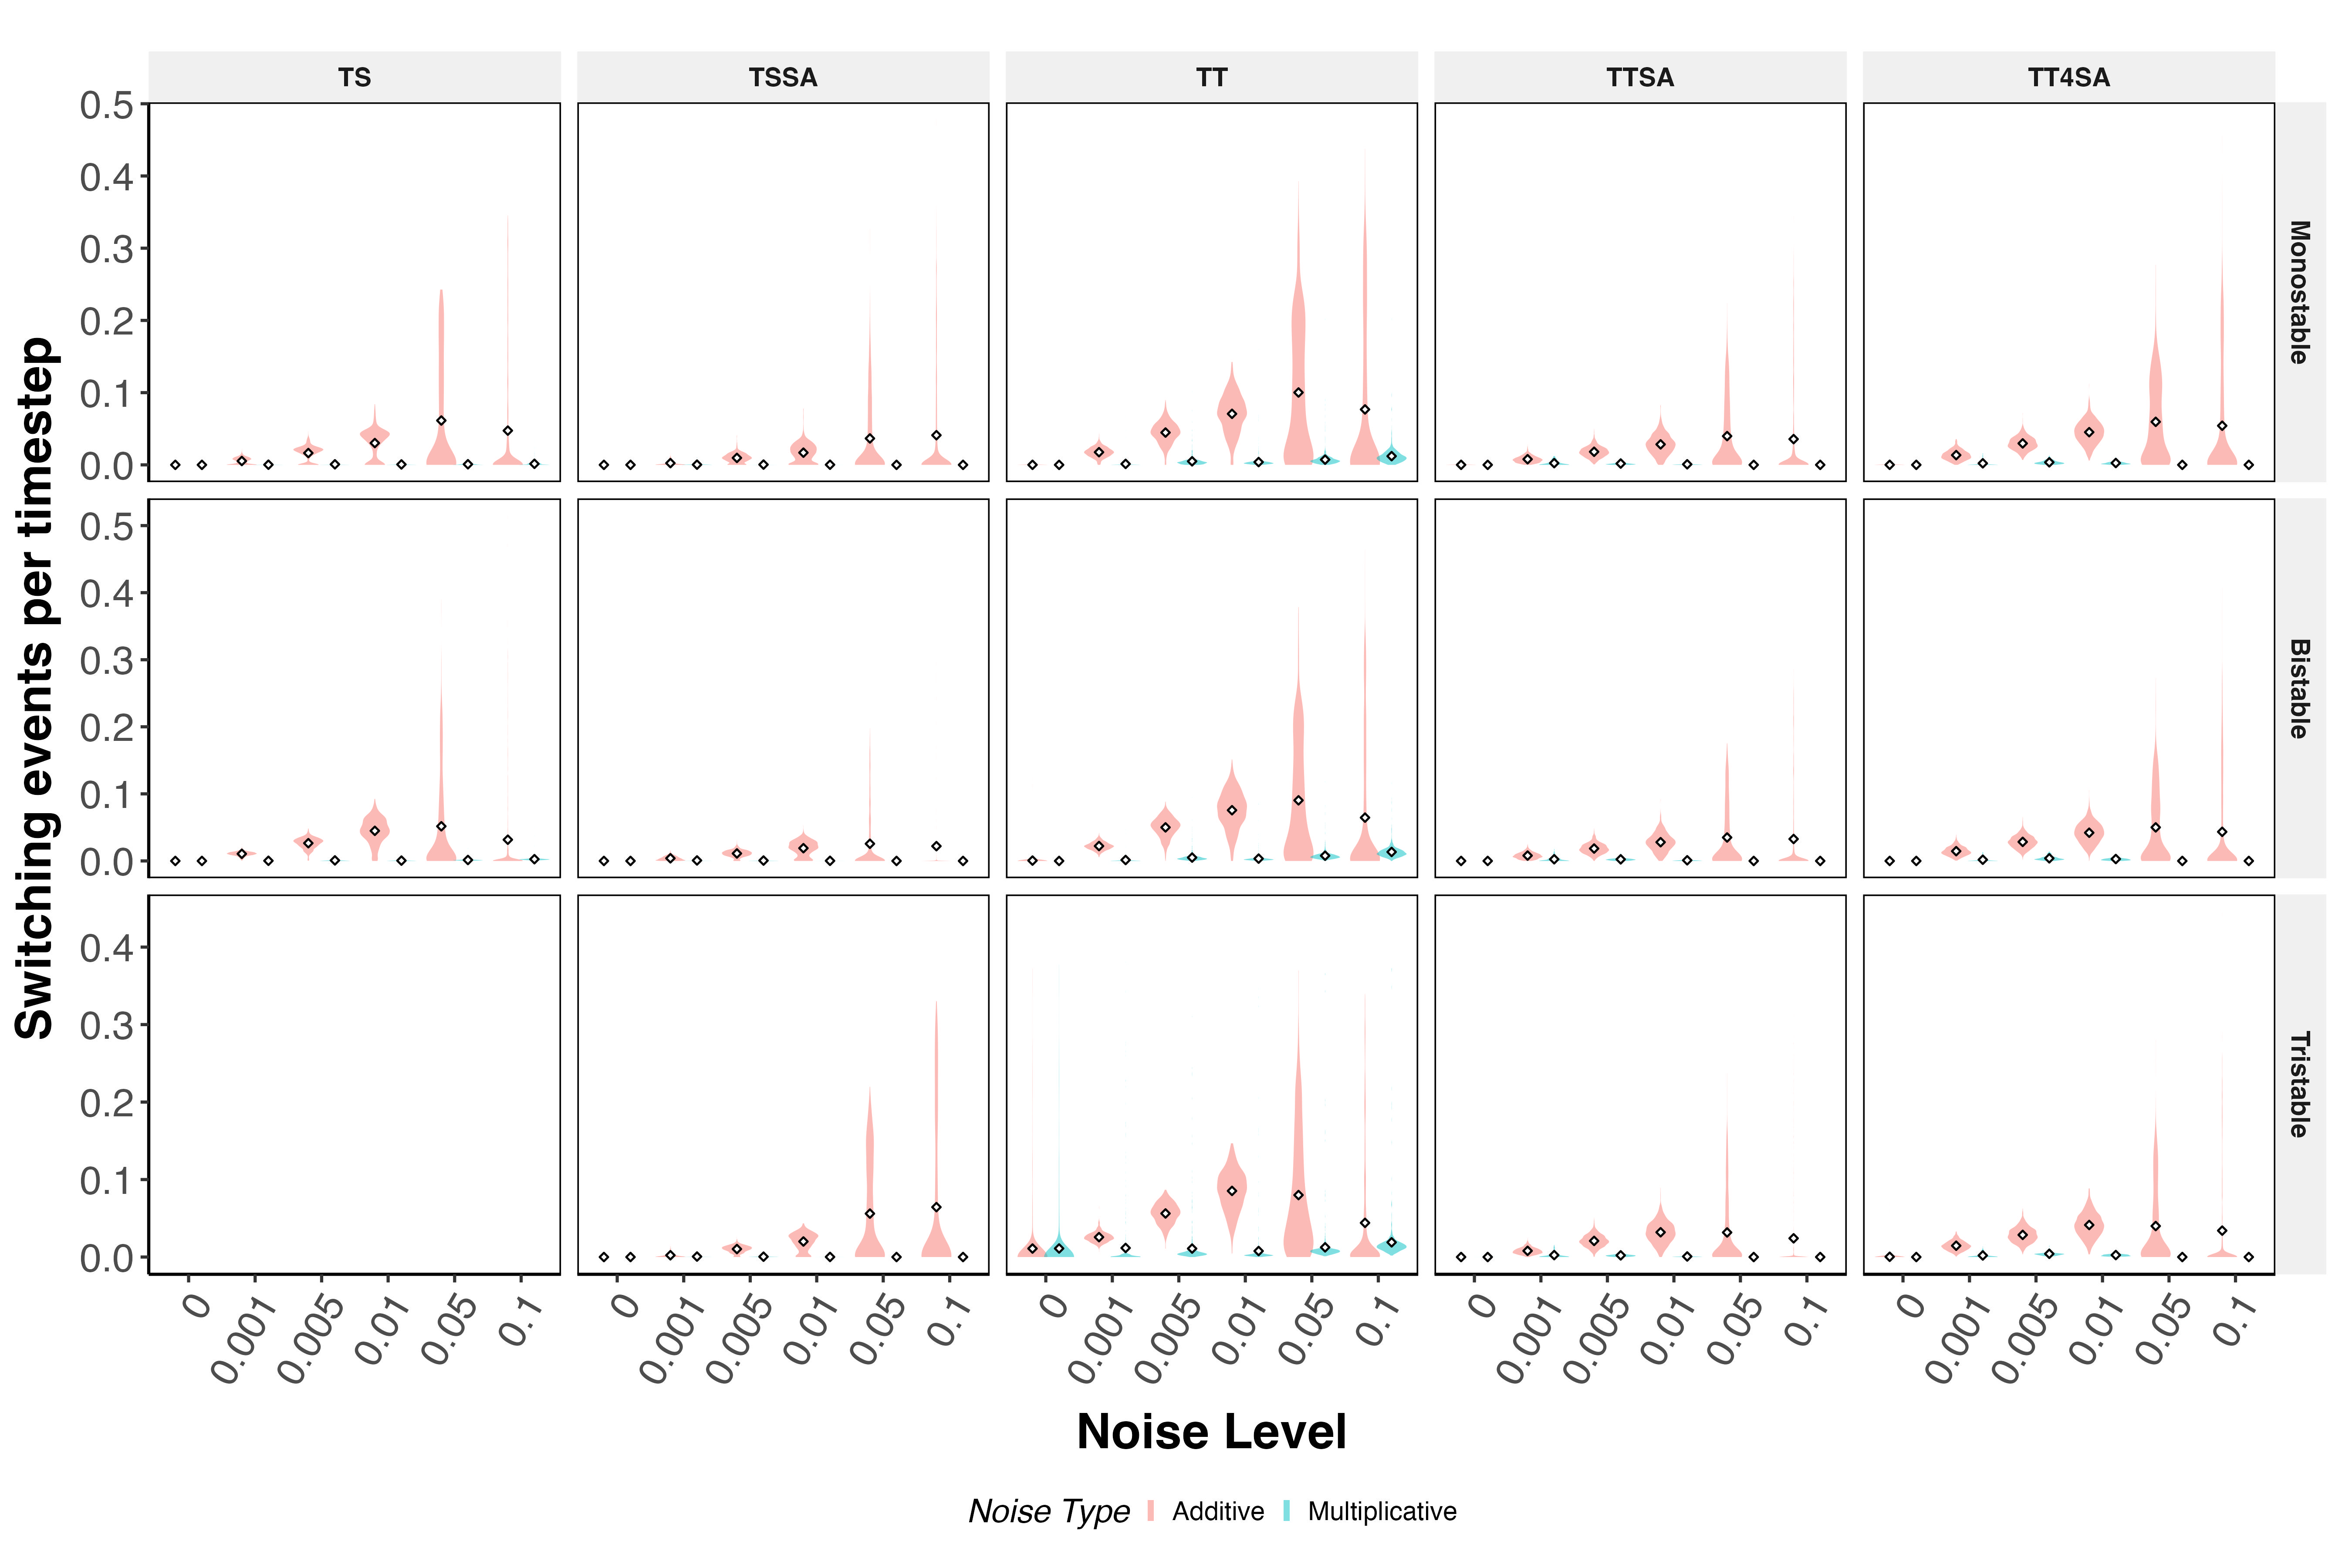
\includegraphics[width=0.8\linewidth]{Fig6S1.jpg}
    \caption{\textbf{Switching-event rates generalize across networks and stability classes.}
    Distribution of switching-event counts per timestep by noise level (Additive vs.\ Multiplicative), for TS, TSSA, TT, TTSA, and TT4SA, faceted by network (columns) and deterministic stability class (rows). TS has no Tristable class (a 2-node network cannot support 3+ distinct stable states), so that facet is empty.
}
    \label{fig:6S1}
\end{figure}

\begin{figure}
    \centering
    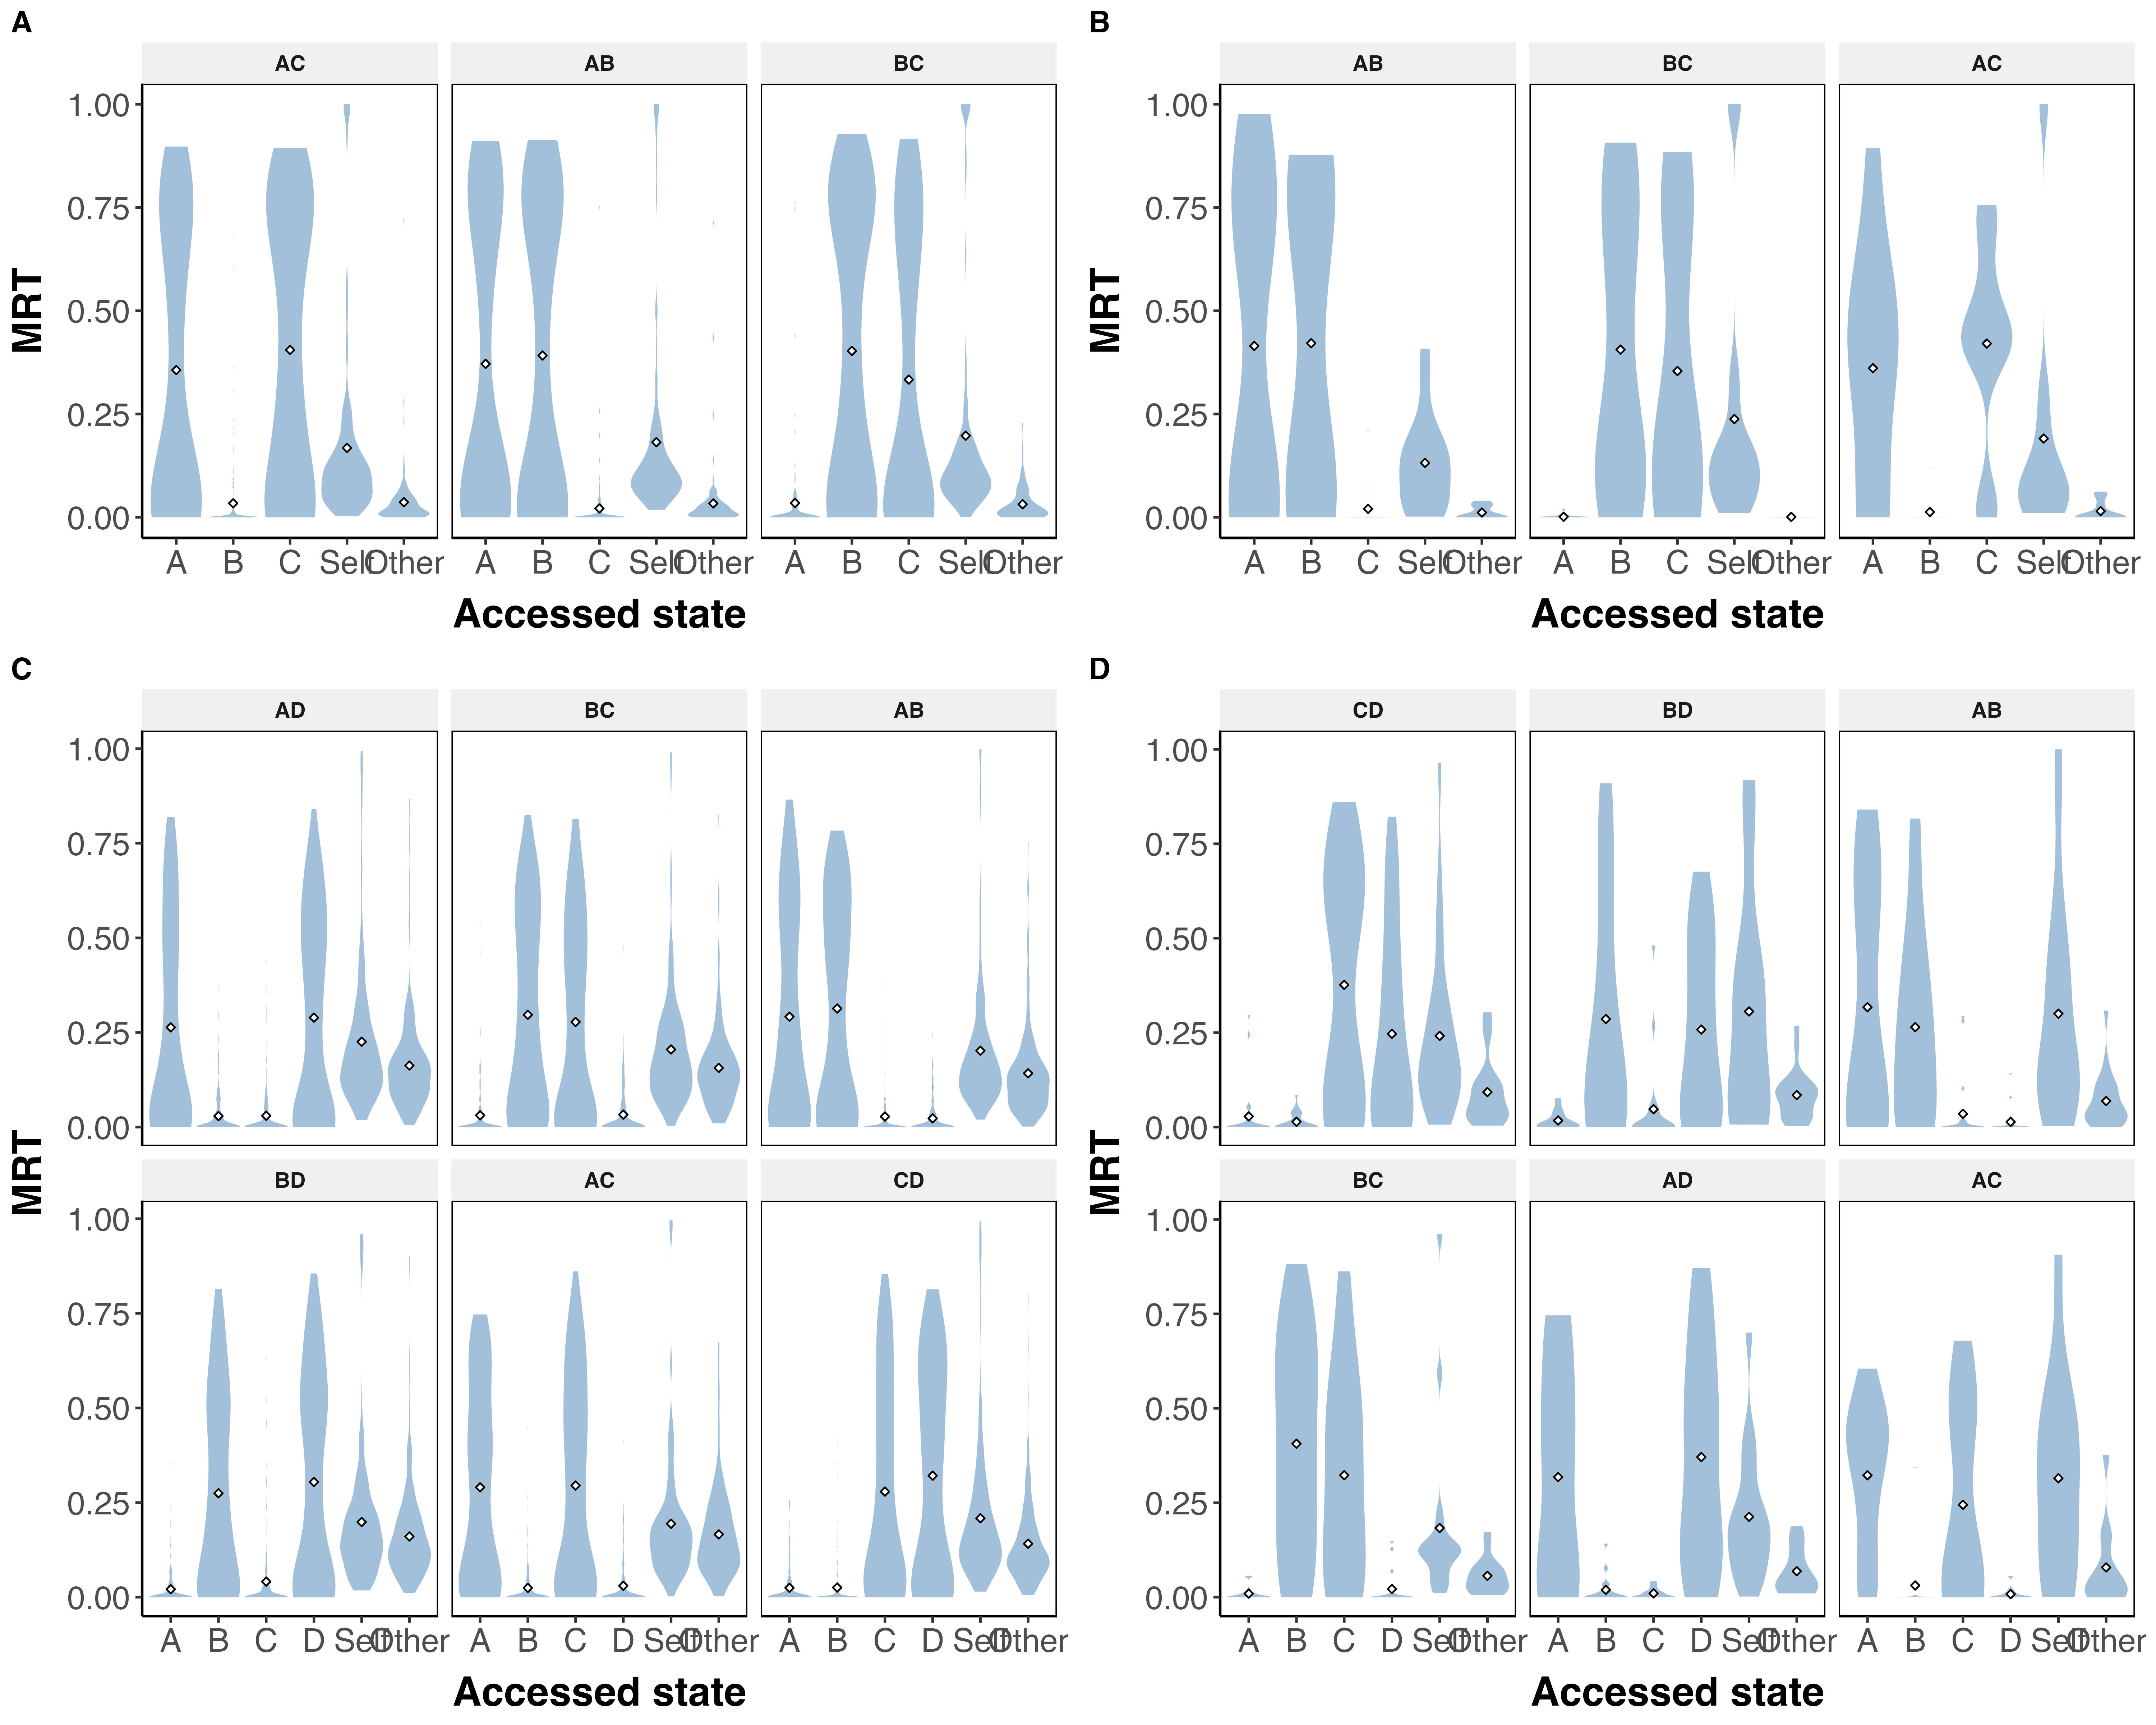
\includegraphics[width=0.8\linewidth]{Fig6S2.jpg}
    \caption{\textbf{Nearest-fate resolution holds for every individual double-high attractor.}
    Per-parameter MRT distribution at noise = 0.01, shown separately for each monostable double-high attractor combination (one facet per combination), for \textbf{(A)} TT, \textbf{(B)} TTSA, \textbf{(C)} TT4, and \textbf{(D)} TT4SA.
}
    \label{fig:6S2}
\end{figure}

\begin{figure}
    \centering
    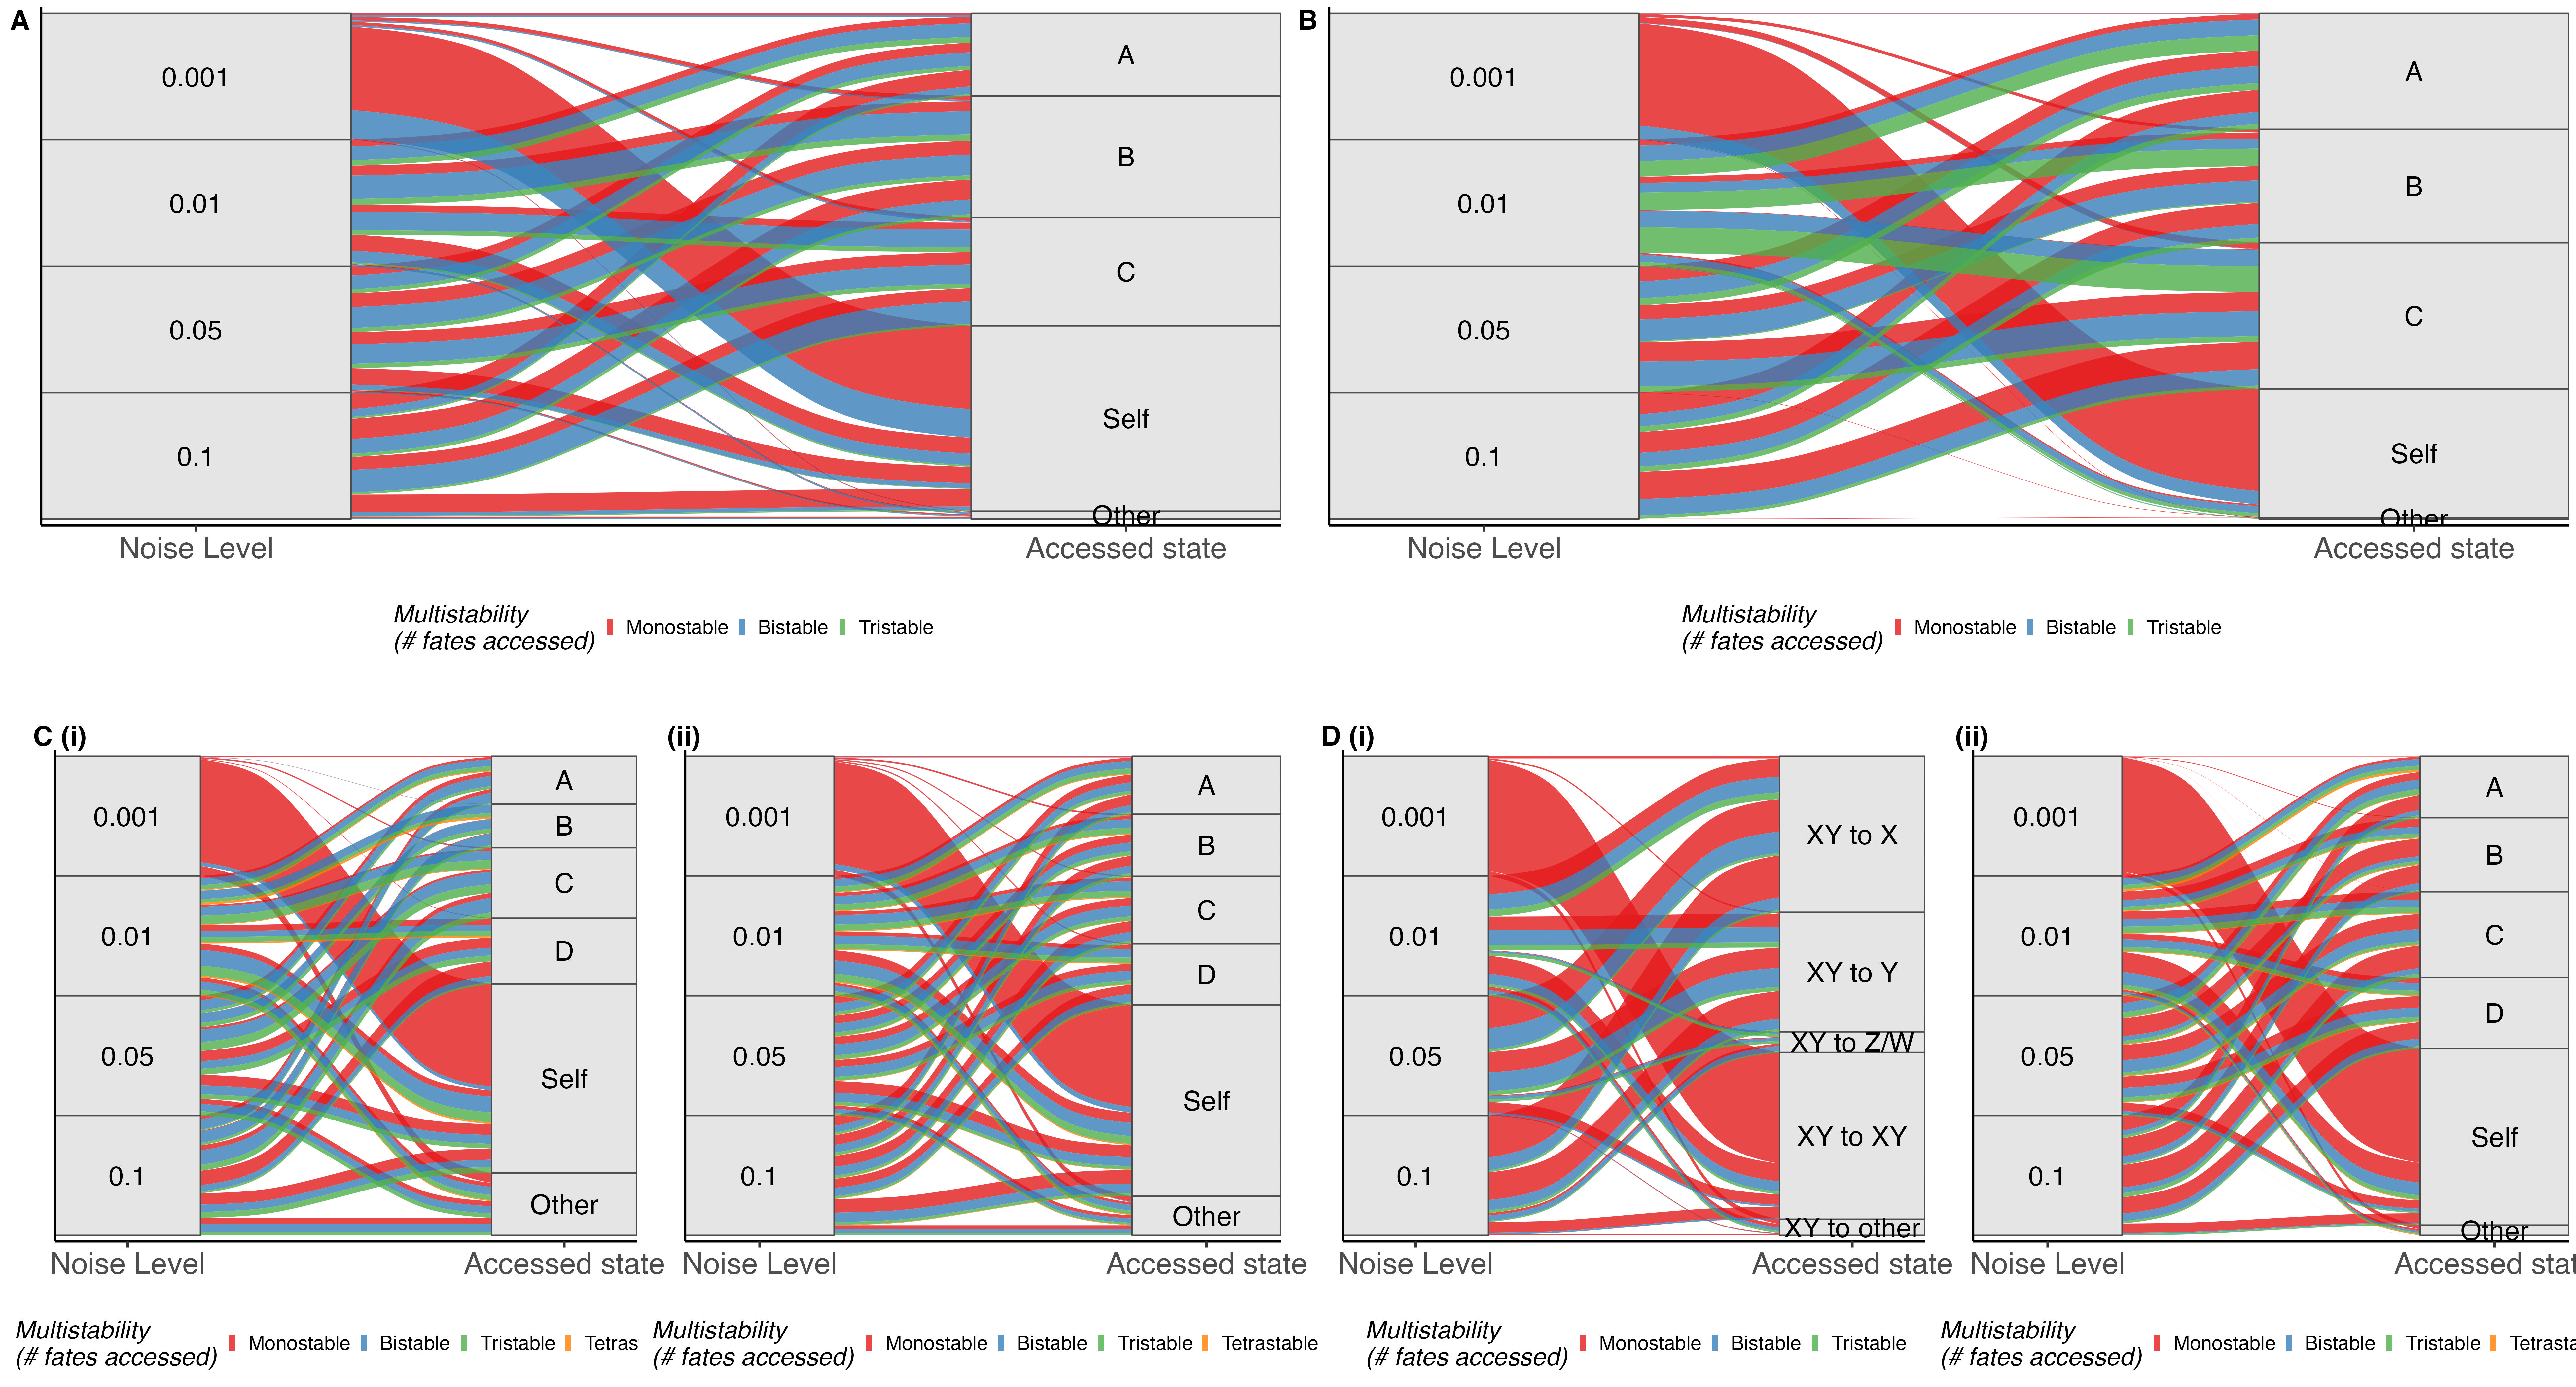
\includegraphics[width=\linewidth]{Fig6S3.jpg}
    \caption{\textbf{Noise-level $\to$ fate alluvials for the bistable double-high classes.}
    Noise-level $\to$ outcome alluvial (as in Figure~\ref{fig:6}E), colored by the multistability classification from Figure~\ref{fig:6}C, for the bistable double-high stability class: \textbf{(A)} TT and \textbf{(B)} TTSA, non-mirror only (mirror bistability is structurally impossible for these 3-node networks). \textbf{(C)} TT4, mirror \textbf{(i)} and non-mirror \textbf{(ii)} shown separately. \textbf{(D)} TT4SA, monostable double-high class \textbf{(i)} (as in Figure~\ref{fig:6}E, for this network) and bistable double-high class \textbf{(ii)}, with mirror and non-mirror populations pooled (TT4SA's mirror-bistable population alone is too sparse, $\approx$13 parameter sets, to interpret on its own).
}
    \label{fig:6S3}
\end{figure}

\begin{figure}
    \centering
    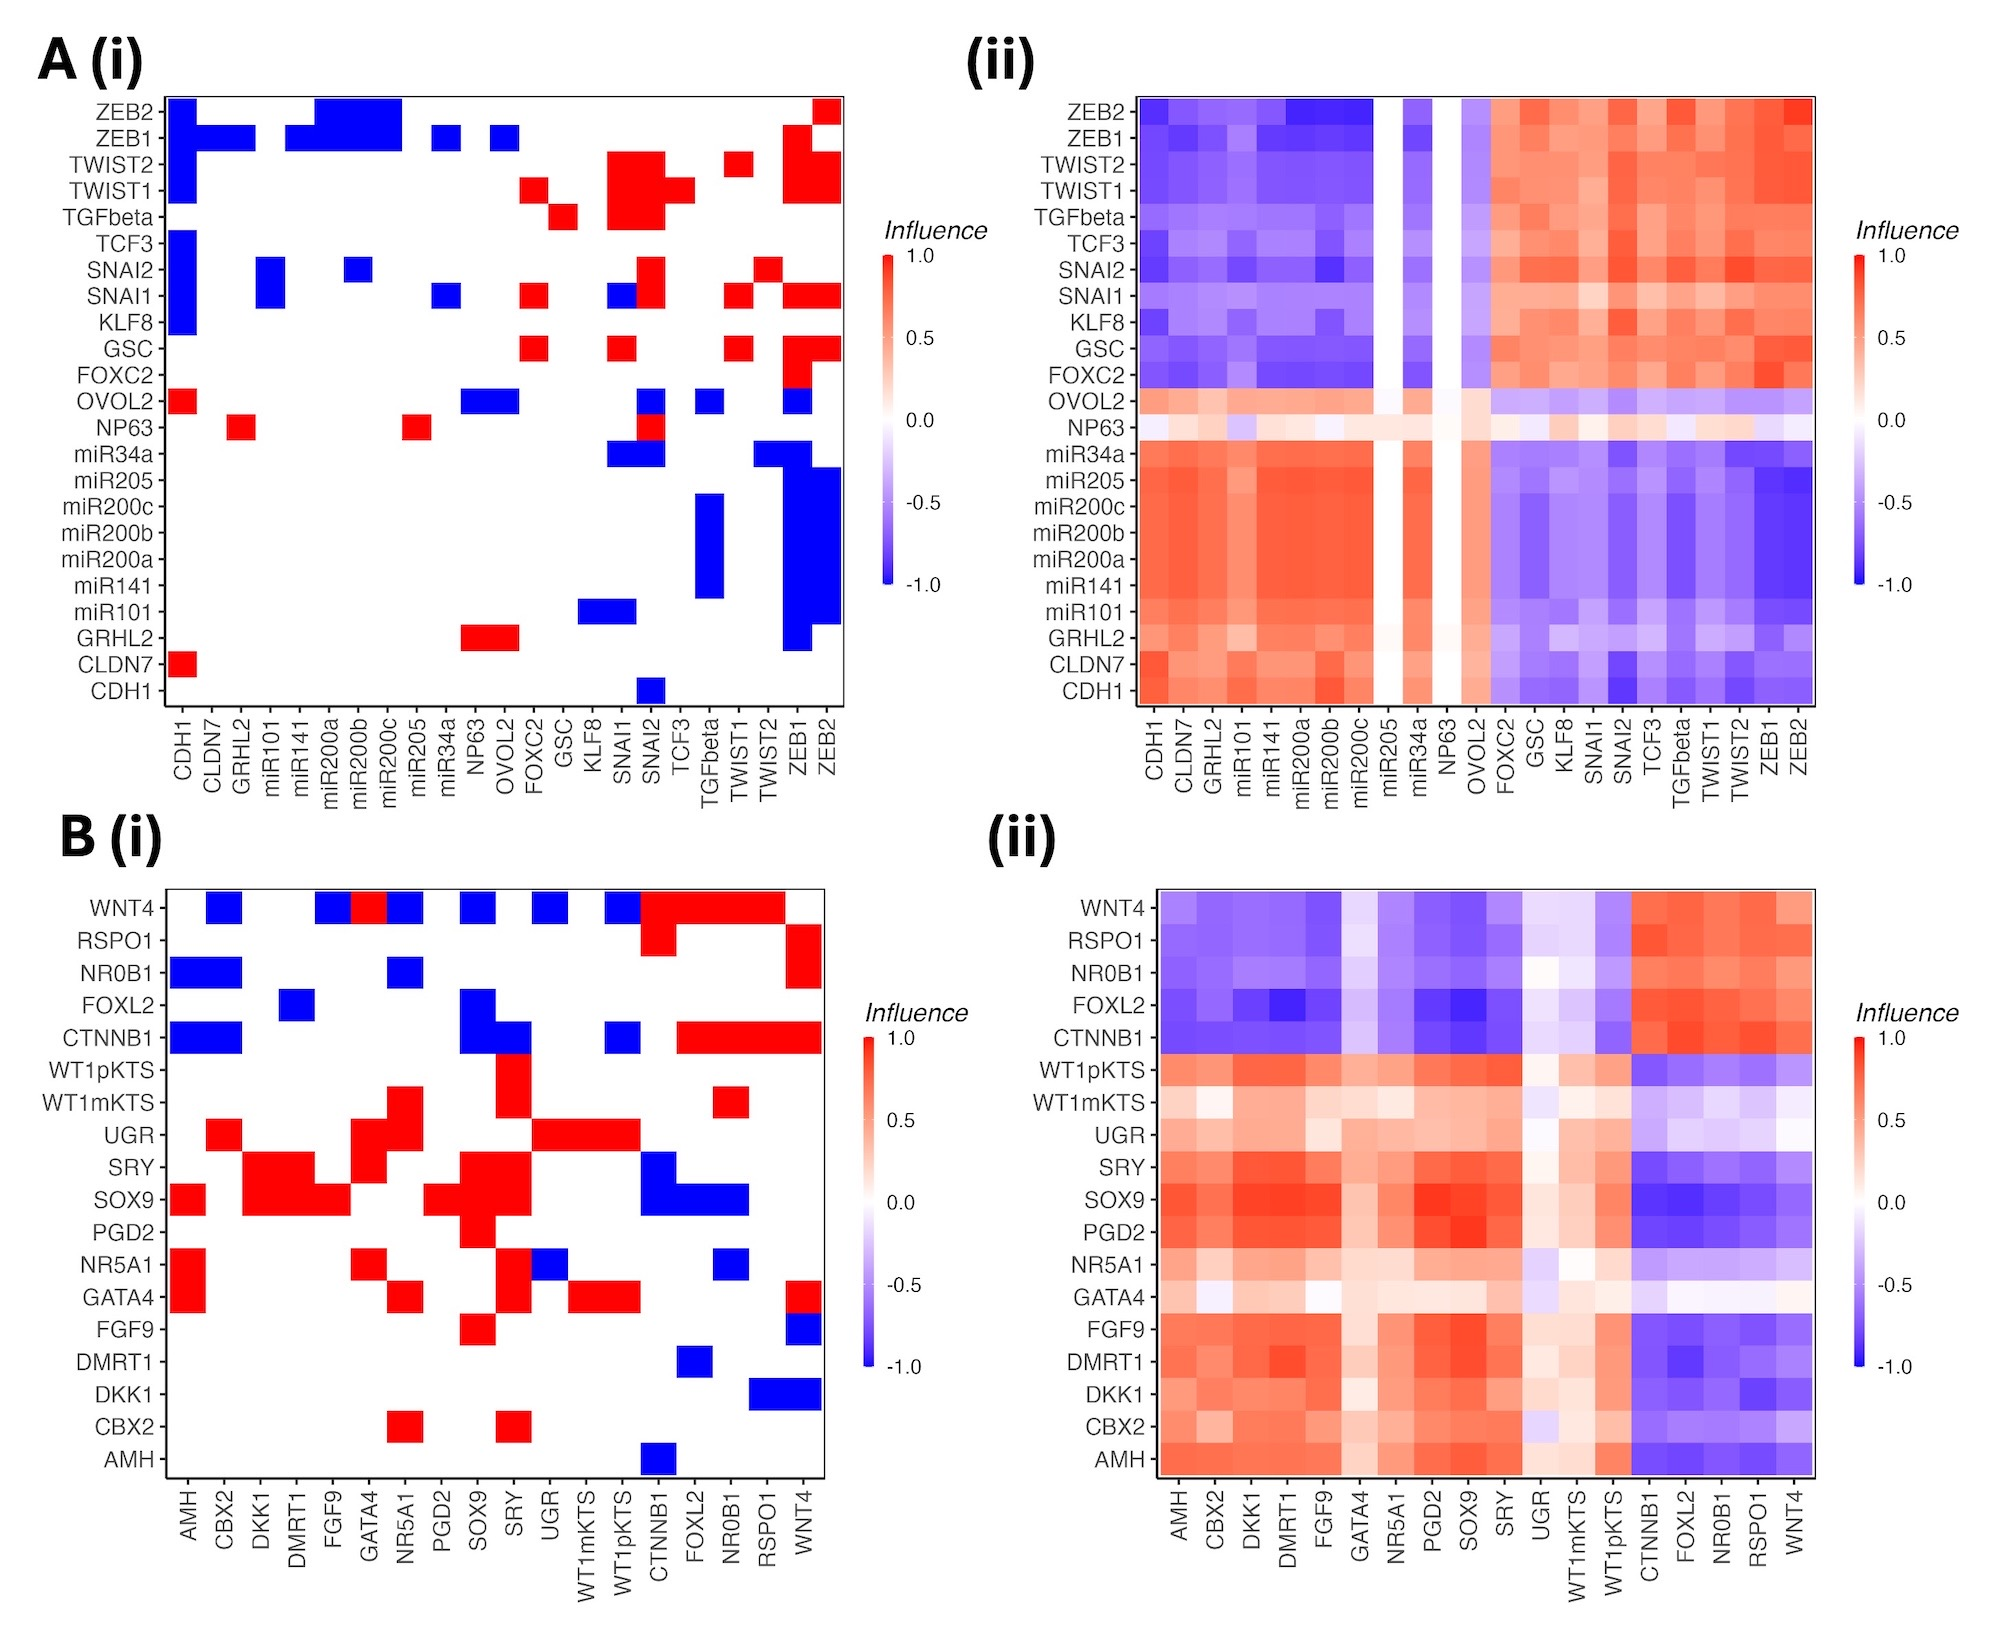
\includegraphics[width=0.8\linewidth]{Fig7S1.jpg}
    \caption{\textbf{Adjacency and influence matrices for the EMT and Gonadal networks.}
    A) EMT network (23 nodes). (i) Direct adjacency matrix showing the signed regulatory
    interactions between node pairs: red indicates activation ($+1$), blue indicates
    inhibition ($-1$), and white indicates no edge. Nodes are ordered by team membership,
    with the epithelial team in the lower-left block and the mesenchymal team in the
    upper-right block. (ii) Influence matrix computed as described in the Methods, showing
    the net cumulative effect between each pair of nodes across all path lengths up to
    $l_{\mathrm{max}} = 10$. Positive (red) values indicate net co-regulation; negative
    (blue) values indicate net counter-regulation. The block structure of the influence
    matrix confirms the two-team organisation of the network.
    B) Gonadal network (19 nodes), displayed in the same format as A, with the
    Sertoli-fate team and the Granulosa-fate team forming the two blocks.}
    \label{fig:7S1}
\end{figure}

\begin{figure}
    \centering
    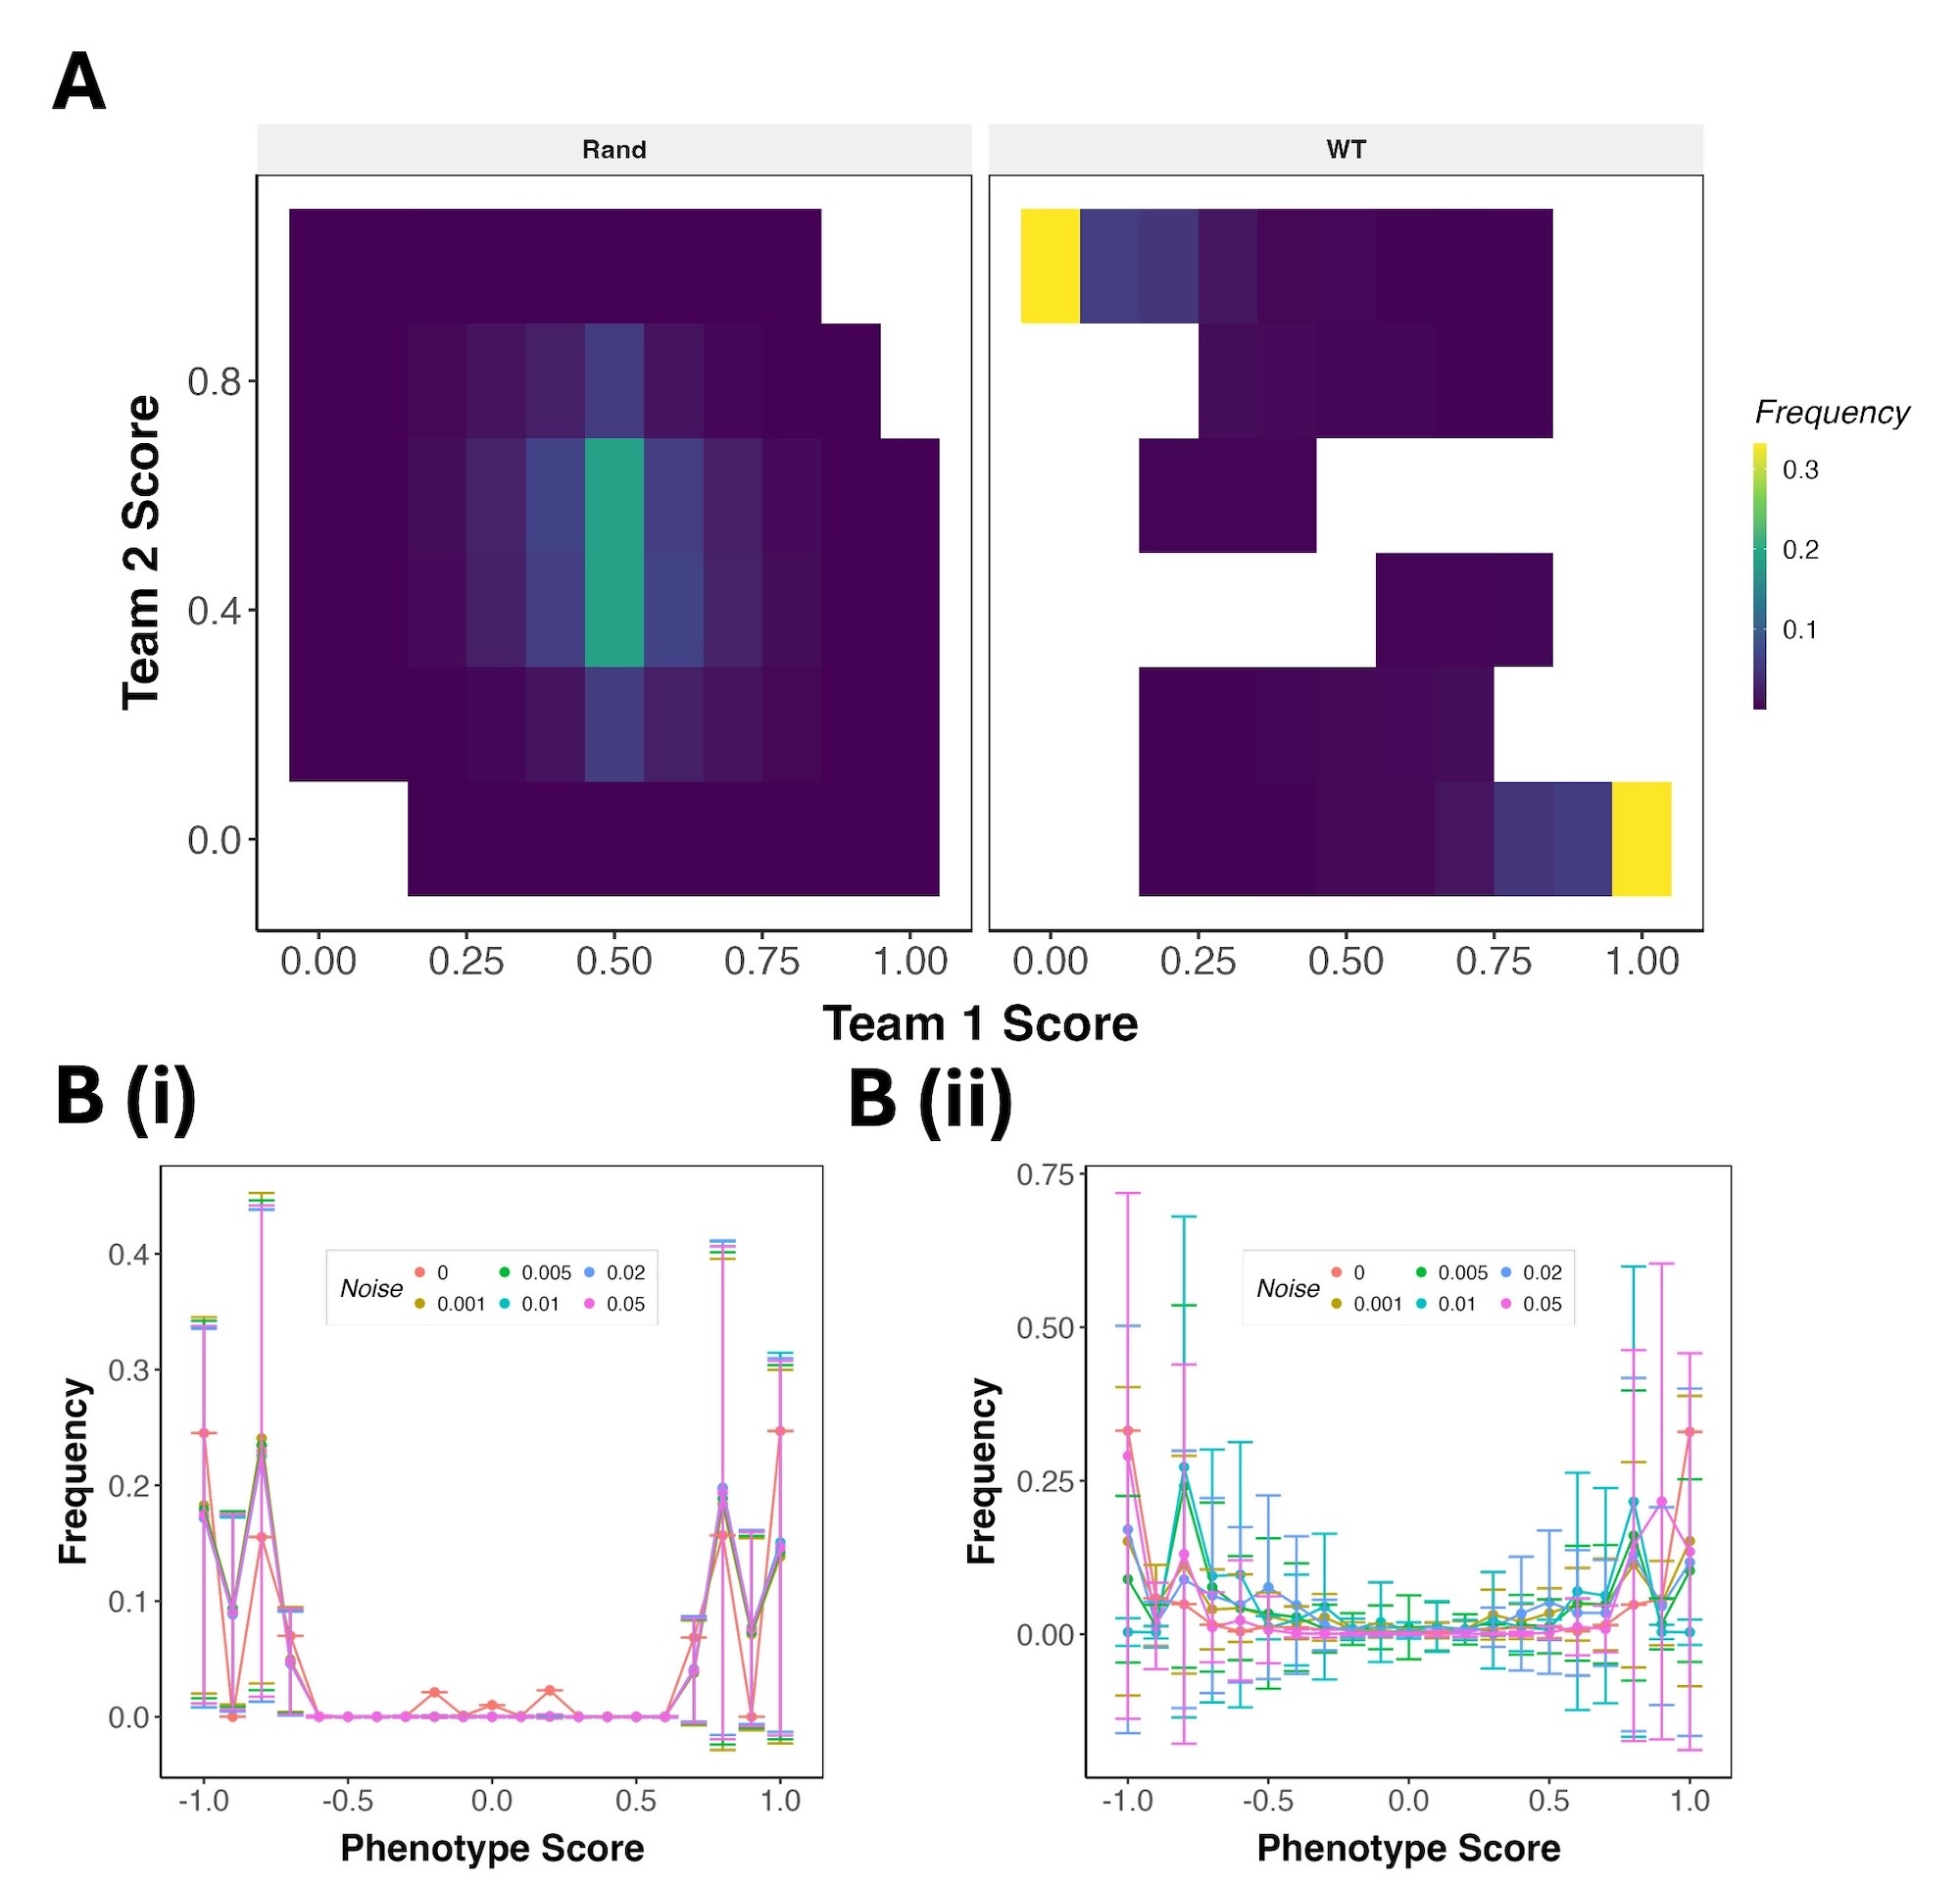
\includegraphics[width=0.8\linewidth]{Fig7S2.jpg}
    \caption{\textbf{Effect of multiplicative and stationary noise on phenotypic
    distributions in biological networks.}
    A) Team score density maps for the Gonadal network under additive noise at
    $\sigma = 0.05$, displayed as in Figure~\ref{fig:4}B. Left panel (``Rand'') shows
    the team score distribution sampled from stochastic simulation trajectories; right
    panel (``WT'') shows the distribution obtained from the steady states of the
    unperturbed network. B) Relative frequency of phenotypic scores across 1000
    simulation trajectories for the Gonadal network under (i) multiplicative noise and (ii) stationary noise.}
    \label{fig:7S2}
\end{figure}
